\documentclass[a4paper, 12pt, oneside]{article}
\usepackage[utf8]{inputenc}
\usepackage[margin=3cm, bindingoffset=1cm]{geometry}
\linespread{1.5}
\usepackage{float}
\usepackage{csquotes}
\usepackage{subfig}
\usepackage{graphicx}
\usepackage{indentfirst}
\usepackage{fancyhdr}
\usepackage{alphabeta}
\usepackage{algpseudocode}
\usepackage{algorithm}
\usepackage{hyperref}
\usepackage[T1]{fontenc}
\usepackage{listings}
\usepackage[htt]{hyphenat}
\usepackage{pgfplots}

\usepackage[
    backend=biber,
    sorting=none
]{biblatex}
\addbibresource{bibliography.bib}


\setlength{\parindent}{1cm}

\pagestyle{fancy}
\fancyhf{}
\fancyhead[C]{\textbf{\leftmark}}
\fancyfoot[C]{\thepage}
\renewcommand{\headrulewidth}{1pt}
\renewcommand{\footrulewidth}{1pt}
\renewcommand{\contentsname}{Indice}
\renewcommand{\figurename}{Figura}

\usepackage[Conny]{fncychap}

  
\begin{document}
\begin{titlepage}
    \begin{center}
        \LARGE{\uppercase{Università degli Studi di Salerno}}\\
        \vspace{5mm}
    	\uppercase{\normalsize Dipartimento di Informatica }\\
    \end{center}
    \begin{figure}[H]
        \centering
        
\includegraphics[width=0.35\textwidth]{logo_unisa}
    \end{figure}
    
    \begin{center}
        \normalsize{Corso di \textbf{Penetration Testing and Ethical Hacking}}\\
    	\vspace{10mm}
    	\LARGE{\textbf{\textsc{NoobBox-1}:\\ Metodologie Utilizzate per il processo di Penetration Testing}}\\
    	\vspace{3mm}
        \large{\uppercase{Anno Accademico 2022/2023}}
    \end{center}

    \vspace{55mm}
    \noindent
    \begin{minipage}[t]{0.6\textwidth}
    	\textsc{Docente}:\\\textbf{Prof. Arcangelo Castiglione}
    	\vspace{10mm}\\
    \end{minipage}
    \hfill
    \begin{minipage}[t]{0.4\textwidth}\raggedleft
    	\textsc{Studente}: \\\textbf{Hermann Senatore}
    \end{minipage}
\end{titlepage}

\tableofcontents
\newpage

\section{Introduzione}
Questo documento si propone di raccogliere in maniera esaustiva tutte le operazioni che sono state compiute allo scopo di condurre l'analisi sull'asset vulnerabile \textsc{NoobBox-1}, disponibile sulla piattaforma VulnHub \cite{noobbox} e che fa uso di un sistema operativo \textbf{GNU\slash Linux}.

Tale documento costituisce il \textbf{Documento 2}, necessario per la consegna dell'attività progettuale del corso di \textbf{Penetration Testing and Ethical Hacking} ed assicura la \textbf{replicabilità} dell'intero processo sulla piattaforma utilizzata.

In particolare, questa sezione consiste una panoramica sull'asset che è stato analizzato e ci si sofferma sull'ambiente utilizzato per condurre l'analisi sull'asset stesso.

\subsection{Ambiente di lavoro ed Information Gathering}
La piattaforma sulla quale è stato svolto l'intero processo consiste in un \textbf{MacBook Air} (late 2020) che utilizza il processore Apple Silicon M1 e che fa uso dell'architettura \textbf{arm64} (aka \textbf{aarch64}).

Per condurre concretamente l'indagine sono state sfruttate due macchine virtuali utilizzando l'\textit{hypervisor} \textbf{UTM}, che utilizza \textbf{QEMU} come suo backend.

In particolare:

\begin{itemize}
    \item La prima macchina virtuale consiste nella versione \textbf{aarch64} del sistema operativo \textbf{Kali Linux};
    \item La seconda macchina virtuale consiste invece nell'asset vulnerabile menzionato poc'anzi.
\end{itemize}.

Di seguito sono presenti alcuni dettagli su entrambe le macchine.

\subsubsection{Macchina virtuale 1: dettagli}
La prima macchina virtuale è stata creata in maniera standard utilizzando l'immagine ISO reperibile presso il sito web della distribuzione \cite{kali}. La versione utilizzata risulta essere la \textbf{2023.1}, rilasciata il 13 marzo 2023. 

In fase di installazione è stato necessario adottare alcuni accorgimenti suggeriti nella relativa documentazione dell'\textit{hypervisor} utilizzato \cite{kali-utm}. Le informazioni presenti in questa pagina sono state create per le versioni \textbf{2022.x} ma sono valide anche per la versione utilizzata durante questo processo.

La macchina virtuale in questione utilizza il kernel Linux 6.1 e di seguito è presente l'output del comando \verb|uname -a|.

\begin{figure}[h]
    \centering
    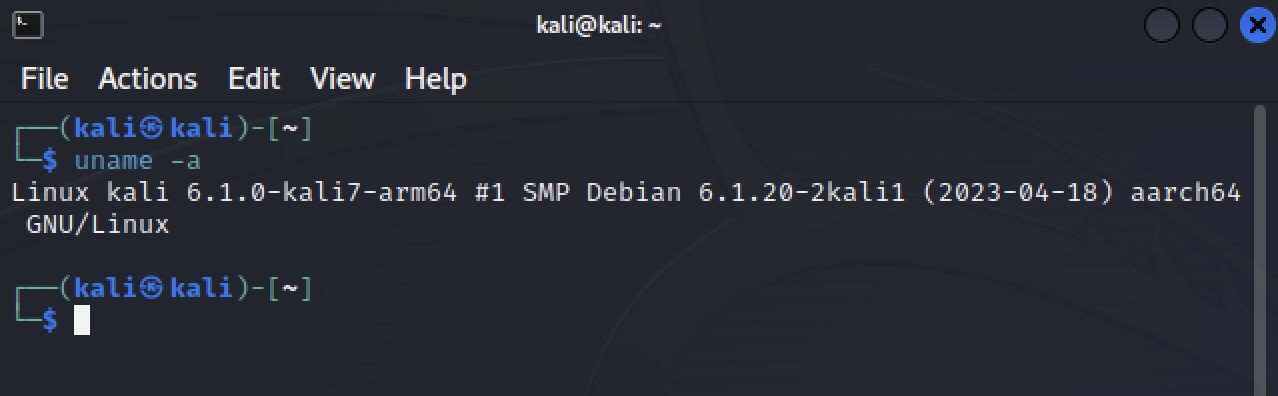
\includegraphics[width=\textwidth]{img/uname.png}
    \caption{La versione del kernel utilizzata da Kali}
\end{figure}

\subsubsection{Dettagli sull'asset}
Come menzionato in precedenza, la seconda macchina consiste proprio nell'asset su cui deve essere condotta l'analisi. Originariamente pensato per essere una sfida CTF, sulla piattaforma VulnHub viene rivelata la presenza di due \textit{flags} a cui accedere: una per l'utente non privilegiato ed una per \texttt{root}. 

Naturalmente, allo scopo di questo progetto non ci si è limitati alla cattura delle flag ma è stato seguito un approccio più sistematico che prevede l'utilizzo di tools e di metodologie standard tipiche di un processo di Penetration Testing.

Sulla piattaforma VulnHub viene offerto il download di NoobBox-1 in formato \texttt{.ova}, compatibile con il software \textbf{Oracle VirtualBox}. Tuttavia, al momento della stesura di questo documento, non esiste una versione nativa di tale software per la piattaforma Apple Silicon in uso e l'hypervisor d'elezione non supporta l'importazione di file \texttt{.ova}. 

Di conseguenza, si è reso necessario un ulteriore step di conversione per rendere tale macchina virtuale utilizzabile con \textbf{UTM} \cite{qcow}. Tale step consiste nella conversione dell'immagine disco in formato \texttt{.vmdk} presente all'interno del file \texttt{.ova} nel formato \texttt{.qcow2}, utilizzato dal software \textbf{QEMU} e quindi da \textbf{UTM}.

Gli step seguiti per la conversione dell'immagine disco sono riportati qui di seguito:

\begin{enumerate}
    \item Installazione di QEMU in maniera \textit{system-wide} usando il package manager \textbf{Homebrew}: \verb|brew install qemu|;
    \item Conversione dell'immagine disco usando il tool \textbf{qemu-img}.
    \begin{center}
        \verb|qemu-img convert -f vmdk -O qcow2 NoobBox-disk001.vmdk NoobBox-disk.qcow2|.
    \end{center}
    Lo switch \texttt{-f} permette di esplicitare il formato \textbf{sorgente}, mentre lo switch \texttt{-O} quello di \textbf{output}.
\end{enumerate}

Successivamente, è stato possibile creare una nuova macchina virtuale \textbf{Linux} e, conseguentemente, importare il file appena creato come disco virtuale.

Al primo avvio della macchina ci si rende conto che è in uso il sistema operativo \textbf{Debian GNU\slash Linux} in versione 10 (codename \texttt{buster}), rilasciato il 6 Luglio 2019. \cite{debian}

In ogni caso, la versione del sistema operativo utilizzato dall'asset sarà oggetto di una successiva analisi per evitare qualsiasi tipo di depistaggio o ambiguità.

La quantità di informazioni che è possibile carpire senza effettuare analisi "esterne" all'asset stesso si ferma tuttavia qui poiché \textbf{non è possibile accedere alla macchina}. Lo scopo della sfida CTF è in reltà proprio quello di effettuare il login e "catturare" le due flag descritte in precedenza. È quindi necessario svolgere ulteriori analisi

Tutti i passaggi descritti in questo documento assumono che la macchina Kali si trovi \textbf{sulla stessa rete locale} della macchina che costituise l'asset da analizzare.

\section{Target Discovery}
Come detto, la diretta conseguenza dell'impossibilità di accedere all'asset in alcun modo consiste nella necessità di determinare in qualche modo il suo indirizzo IP sulla rete.

L'hypervisor UTM crea come impostazione predefinita una rete \textbf{NAT} che usa il range (qui riportato in notazione CIDR) \textbf{192.168.64.0\slash24}.

Prima di tutto, è necessario specificare che:

\begin{itemize}
    \item Anche la macchina Host (su cui è in esecuzione l'hypervisor) fa parte della rete NAT ed ha indirizzo IP \textbf{192.168.64.1} sull'interfaccia \texttt{bridge100};
    \item La macchina Kali ha come indirizzo \textbf{192.168.64.15} sull'interfaccia \texttt{eth0}.
\end{itemize}

A questo punto, per determinare l'indirizzo IP dell'asset è possibile utilizzare il tool \texttt{netdiscover}, che viene fornito di default con Kali Linux e che deve essere eseguito come utente \texttt{root}.

Suddetto tool, secondo la documentazione accessibile mediante il comando \texttt{man netdiscover}, permette di rilevare host attivi su di una rete locale inviandogli richeste \textbf{ARP}. 

Due sono le opzioni che devono essere specificate in questo contesto:

\begin{itemize}
    \item \texttt{-i eth0} permette di utilizzare l'interfaccia di rete \texttt{eth0};
    \item \texttt{-r 192.168.64.0\slash24} permette invece di specificare il range di indirizzi compreso tra 192.168.64.0 e 192.168.64.255, specificato in notazione CIDR.
\end{itemize}

\newpage
L'output per
\begin{center}
    \texttt{netdiscover -i eth0 -r 192.168.64.0\slash24}
\end{center}

viene riportato qui di seguito.

\begin{figure}[h]
    \centering
    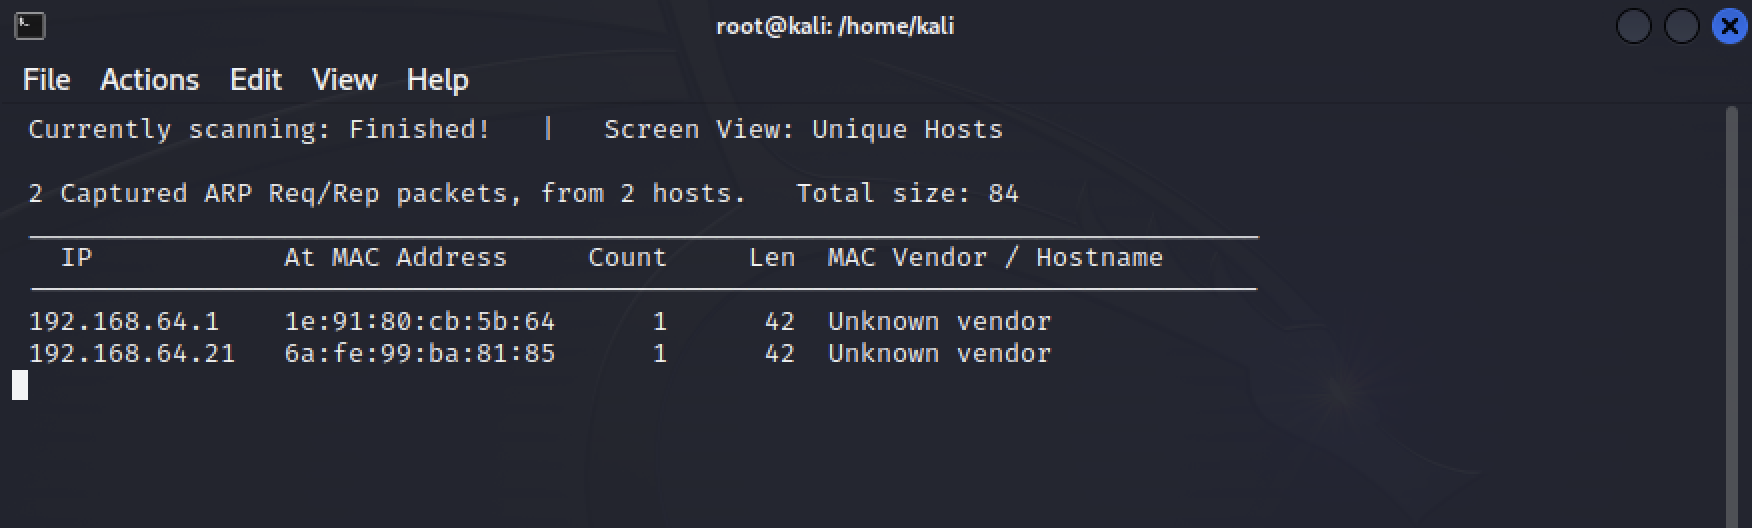
\includegraphics[width=\textwidth]{img/netdiscover.png}
    \caption{L'output di \texttt{netdiscover}}
\end{figure}

Tralasciando l'host 192.168.64.1 che si è menzionato appartenere alla macchina fisica che ospita l'hypervisor, è possibile notare la presenza di un host attivo con indirizzo 192.168.64.21 e, dato che al momento dell'esecuzione del tool non erano in esecuzione altre macchine virtuali oltre all'asset in analisi, è possibile concludere che \textbf{192.168.64.21} sia effettivamente \textbf{il suo indirizzo}.

\subsection{Probing della macchina}

Una volta ottenuto l'indirizzo IP della macchina, è ora necessario cercare di capire se la macchina identificata sia effettivamente raggiungibile in qualche modo. In questa sezione, viene sfruttato il tool \texttt{ping} che sfrutta il meccanismo degli \textbf{ICMP Echo Request\slash Reply}.

La sintassi del comando ping, come specificato nella relativa documentazione, prevede la specifica di un indirizzo IP da contattare, ed eventualmente (mediante lo switch \texttt{-c}) il numero di richieste da inoltrare al target da analizzare. In questo contesto, al target verranno inoltrare 3 richieste ICMP. Il comando eseguito risulta quindi essere:

\begin{center}
    \texttt{ping -c 3 192.168.64.21}
\end{center}

\begin{figure}[h!]
    \centering
    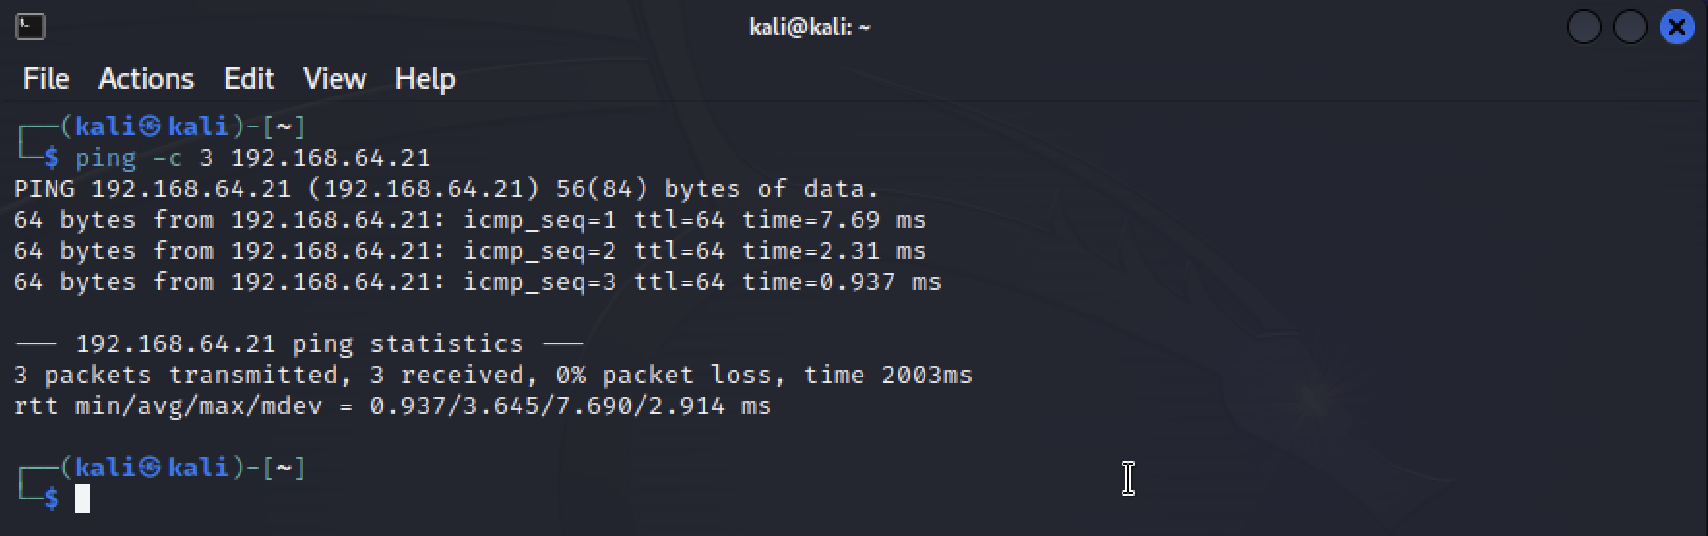
\includegraphics[width=\textwidth]{img/ping.png}
    \caption{L'output di \texttt{ping}}
\end{figure}

Senza adottare particolari accorgimenti, dall'output del comando mostrato qui sopra è possibile notare come la macchina in questione sia effettivamente \textbf{raggiungibile dall'esterno}, almeno utilizzando il protocollo ICMP.

\subsection{OS Fingerprinting}
Il passo successivo dell'analisi condotta consiste nell'identificare con certezza ed in maniera non ambigua il sistema operativo utilizzato dall'asset. A questo scopo, è possibile far riferimento ai tool \texttt{p0f} ed \texttt{nmap}, quest'ultimo utilizzato anche nelle fasi successive dell'analisi.

\subsubsection{\texttt{p0f}}
Il tool \textbf{\texttt{p0f}} utilizza una \textbf{tecnica di fingerprinting} basata sull'analisi della composizione dei pacchetti \textbf{TCP\slash IP} provenienti dalla macchina target per determinare \textbf{passivamente} il suo sistema operativo\cite{p0f}. L'utilizzo del tool prevede l'esecuzione come utente root. Una volta avviato, si mette in ascolto sull'interfaccia specificata dallo switch \texttt{-i} (in questo caso \texttt{eth0}), catturerà i pacchetti e restituirà informazioni sull'host che ha generato quel determinato pacchetto. Si rivela quindi necessaria la \textbf{generazione} di traffico verso il target per condurre l'analisi in questione. 

Il comando completo utilizzato in questo contesto risulta essere:

\begin{center}
    \texttt{p0f -i eth0}
\end{center}

Come prima cosa, si è provato ad accedere all'asset mediante il comando \texttt{curl} utilizzando l'indirizzo IP ottenuto in precedenza sulla porta 80, che in questo caso si è rivelata \textbf{aperta}.\footnote{Si tenga presente che lo stato della porta 80 costituisce già di per sé un elemento \textbf{prezioso} per l'indagine in corso, ma una discussione approfonditta su questo topic verrà affrontata nella sezione dedicata alla \textbf{Target Enumeration}}.


Analizzando tuttavia i risultati mostrati a schermo (qui di seguito, si notino i punti interrogativi in corrispondenza della voce \texttt{server}) ci si accorge che il tool \texttt{p0f} \textbf{non è riuscito ad identificare correttamente il sistema operativo del target}. Si è reso quindi necessario provare altre strategie.

\begin{figure}[h!]
    \centering
    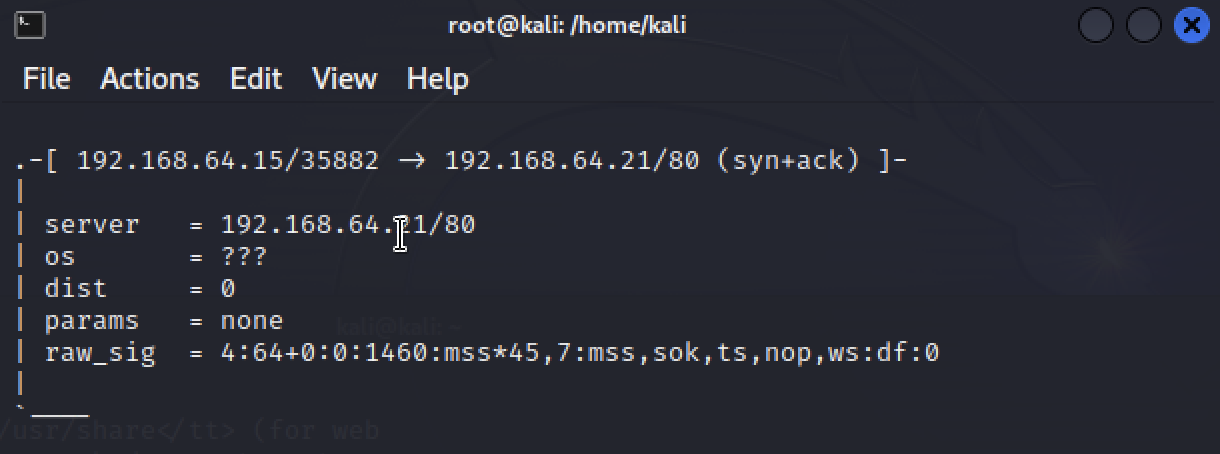
\includegraphics[width=\textwidth]{img/p0f.png}
    \caption{L'output di \texttt{p0f}. L'indirizzo IP \texttt{192.168.64.15} appartiene alla macchina Kali.}
\end{figure}

\subsubsection{\texttt{nmap}}
\texttt{nmap} è probabilmente uno dei tool più conosciuti ed utilizzati per condurre operazioni di Target Enumeration (ed infatti verrà utilizzato principalmente in questa fase per effettuare l'operazione di \textbf{port scanning}) e di security auditing in generale ma che può essere utilizzato anche per effettuare OS Fingerprinting.\cite{nmap}

Suddetta operazione può essere effettuata mediante lo switch \texttt{-O} in combinazione con l'host da scansionare. La command line completa utilizzata in questo caso è la seguente:

\begin{center}
    \texttt{nmap -O 192.168.64.21}
\end{center}

Di seguito viene riportato il risultato della scansione.

\begin{figure}[h!]
    \centering
    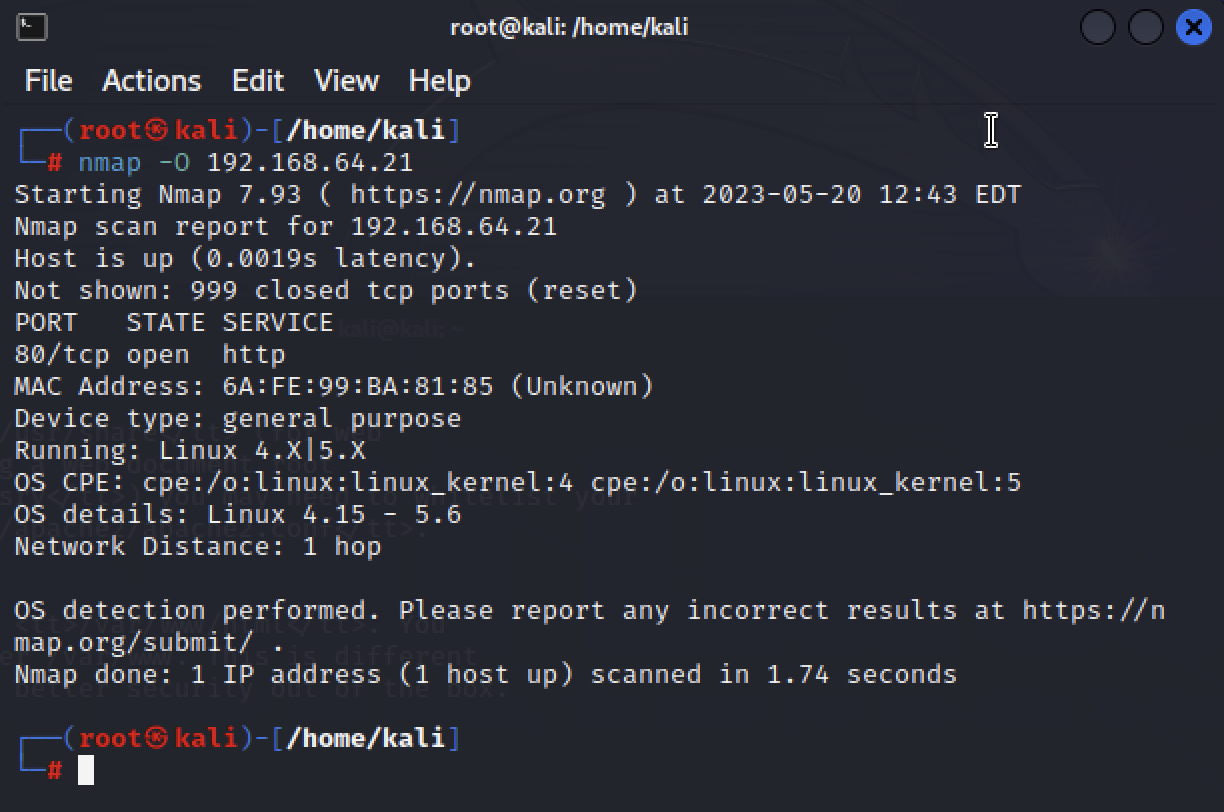
\includegraphics[width=\textwidth]{img/nmap-os.png}
    \caption{L'output di \texttt{nmap}.}
\end{figure}

Secondo \texttt{nmap}, il target consiste in una macchina \textbf{general purpose} che utilizza il kernel \textbf{Linux} in una versione compresa tra la \textbf{4.15} e la \textbf{5.6}. Considerando che Debian 10 è stato rilasciato con il kernel \textbf{4.19} \cite{debian}, è possibile concludere che le informazioni ottenute in precedenza risultano \textbf{corrette}. Si noti come \texttt{nmap} abbia inoltre rilevato la porta 80 come \textbf{aperta}.

\section{TCP Port Scanning e Target Enumeration}

Nella fase precedente, oltre all'estrazione di diverse informazioni sul target, è stata ricavata anche un'altra, importante, informazione circa lo stato di apertura della porta \texttt{tcp/80}. Il fatto che la porta 80 sia aperta fa presupporre che sul target sia in esecuzione un qualche tipo di servizio web. Questa sezione, definita di \textbf{Target Enumeration}, approfondisce questa ipotesi e conduce un'analisi sistematica riguardo ai servizi in esecuzione sul target mediante il tool \texttt{nmap}, stavolta utilizzato nel suo contesto principale.

In particolare, il tool \texttt{nmap} sarà utilizzato per:

\begin{itemize}
    \item Scansionare tutte le 65535 porte del target (switch \texttt{-p-});
    \item Identificare la versione dei servizi attivi (switch \texttt{-sV});
    \item Esportare i risultati della scansione in formato XML nel file \texttt{nmap\_noobbox\_report.xml} (switch \texttt{-oX nmap\_noobbox\_report.xml}).
\end{itemize}

Il comando utilizzato quindi risulta essere:

\begin{center}
    \texttt{nmap -p- -sV 192.168.64.1 -oX nmap\_noobbox\_report.xml}
\end{center}

In questo caso, avendo a disposizione l'accesso root alla macchina Kali, è stato utilizzata la cosiddetta \textbf{SYN Scan} (switch \texttt{-sS}, ma che essendo la scansione di default è stato omesso dalla command line).

Di seguito è riportato l'output del tool.

\begin{figure}[h!]
    \centering
    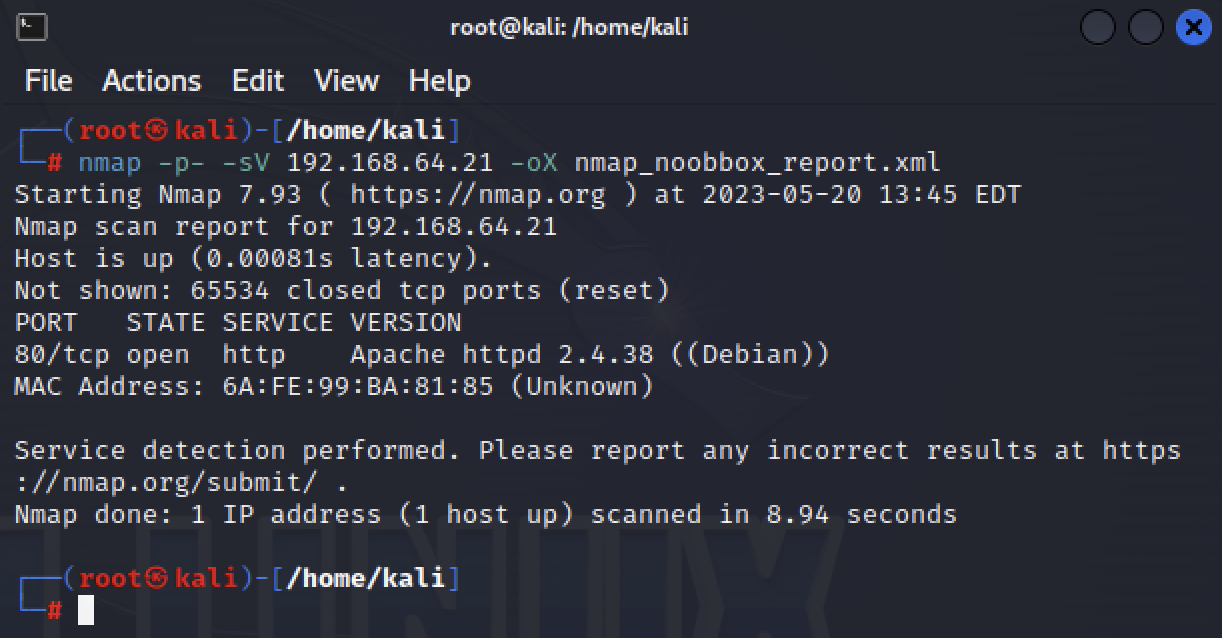
\includegraphics[width=\textwidth]{img/nmap-enum.png}
    \caption{L'output di \texttt{nmap}.}
\end{figure}

In allegato al presente documento è presente il report generato da \texttt{nmap} e convertito in HTML mediante il tool \texttt{xsltproc}, chiamato \texttt{nmap\_noobbox\_report.html}.

\subsection{TCP Port Scanning: Analisi dei risultati}
Facendo riferimento al report generato è possibile notare che:

\begin{itemize}
    \item Il servizio presente sulla porta 80 TCP (identificata come aperta anche in precedenza) consiste in \textbf{Apache \texttt{httpd}} in versione \textbf{2.4.38};
    \item Non è presente nessun altro servizio TCP attivo sul target, dato che le altre 65534 porte sono state dichiarate \textbf{chiuse};
    \item È stato possibile ottenere un ulteriore discontro sul sistema operativo in esecuzione sull'asset: \textbf{Debian}.
\end{itemize}

\subsection{Extra: UDP Port Scanning}
La scansione effettuata in precedenza tramite \texttt{nmap} ha determinato lo stato di apertura delle 65535 porte \textbf{TCP}. Per completezza, sarà ripetuta la stessa scansione delle 65535 porte stavolta usando il protocollo \textbf{UDP}. Il tool utilizzato in questo contesto consiste in \texttt{unicornscan}. Questo tool non è presente nell'installazione di default di Kali Linux, ma è possibile installarlo (insieme alle relative dipendenze) mediante il comando:

\begin{center}
    \texttt{sudo apt install unicornscan}
\end{center}

La sintassi di \texttt{unicornscan} \cite{unicornscan} è abbastanza simile a quella utilizzata da \texttt{nmap}. In questo caso, il tool verrà utilizzato per:

\begin{itemize}
    \item Effettuare una scansione \textbf{UDP} (switch \texttt{-m U});
    \item Scansionare le 65535 porte dell'asset con indirizzo IP 192.168.64.21 (usando la sintassi \texttt{192.168.64.21:1-65535});
    \item Ottenere un output \textit{prolisso} (switch \texttt{-Iv});
    \item Inviare 2000 pacchetti al secondo (più veloce rispetto ai 300 pacchetti al secondo di default) (switch \texttt{-r 2000}).
\end{itemize}

Riassumendo:

\begin{center}
    \texttt{unicornscan -m U 192.168.64.21:1-65535 -Iv -r 2000}
\end{center}

Di seguito viene riportato l'output del comando precedente.

\begin{figure}[h!]
    \centering
    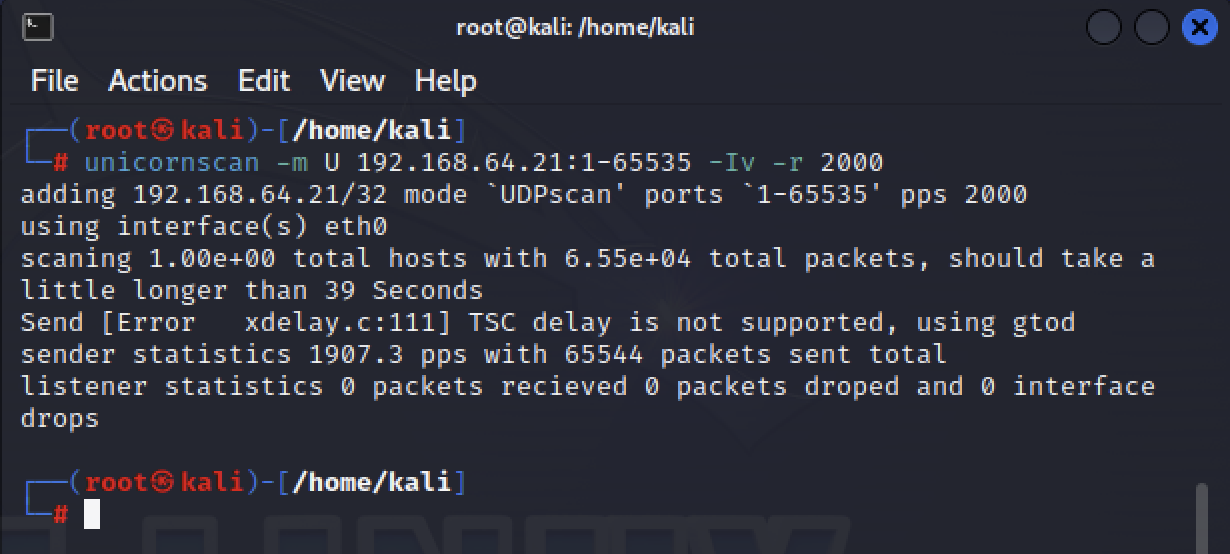
\includegraphics[width=\textwidth]{img/unicornscan.png}
    \caption{L'output di \texttt{unicornscan}.}
\end{figure}

\subsubsection{UDP Port scanning: analisi dei risultati}
Consultando l'output del comando, ci si rende conto che sull'asset \textbf{non sia presente} alcun servizio attivo su \textbf{nessuna} porta UDP.

Si noti il messaggio di errore relativo al delay. Secondo la \textit{manpage} \cite{unicornscan-man}, il tool di default sfrutta il timer \textbf{TSC} per gestire il delay tra l'invio dei vari pacchetti. Quando questo timer non è disponibile, il tool ne utilizza un altro: \textbf{GTOD}. 

Il timer TSC è presente su quasi tutte le CPU \textbf{x86} ed \textbf{x86\_64} con quella denominazione, ma non sulle CPU basate sull'architettura \textbf{aarch64}, come quella utilizzata per condurre l'indagine. 

La scansione con \textbf{unicornscan} ha quindi utilizzato il timer \textbf{GTOD}, senza particolari differenze all'atto pratico.

\subsection{Analisi del server web}
Uno dei risultati principali della fase di port scanning consiste nell'aver scoperto che la porta 80 sia \textbf{aperta}. Dall'analisi condotta mediante \texttt{nmap} è stato appurato che sulla porta 80 sia attivo il web server \textbf{Apache \texttt{httpd}}. 

Visitando la pagina \texttt{http://192.168.64.21/} dalla macchina Kali, viene infatti presentata la pagina di default del web server quando installato su \textbf{Debian}.
\newpage

\begin{figure}[h!]
    \centering
    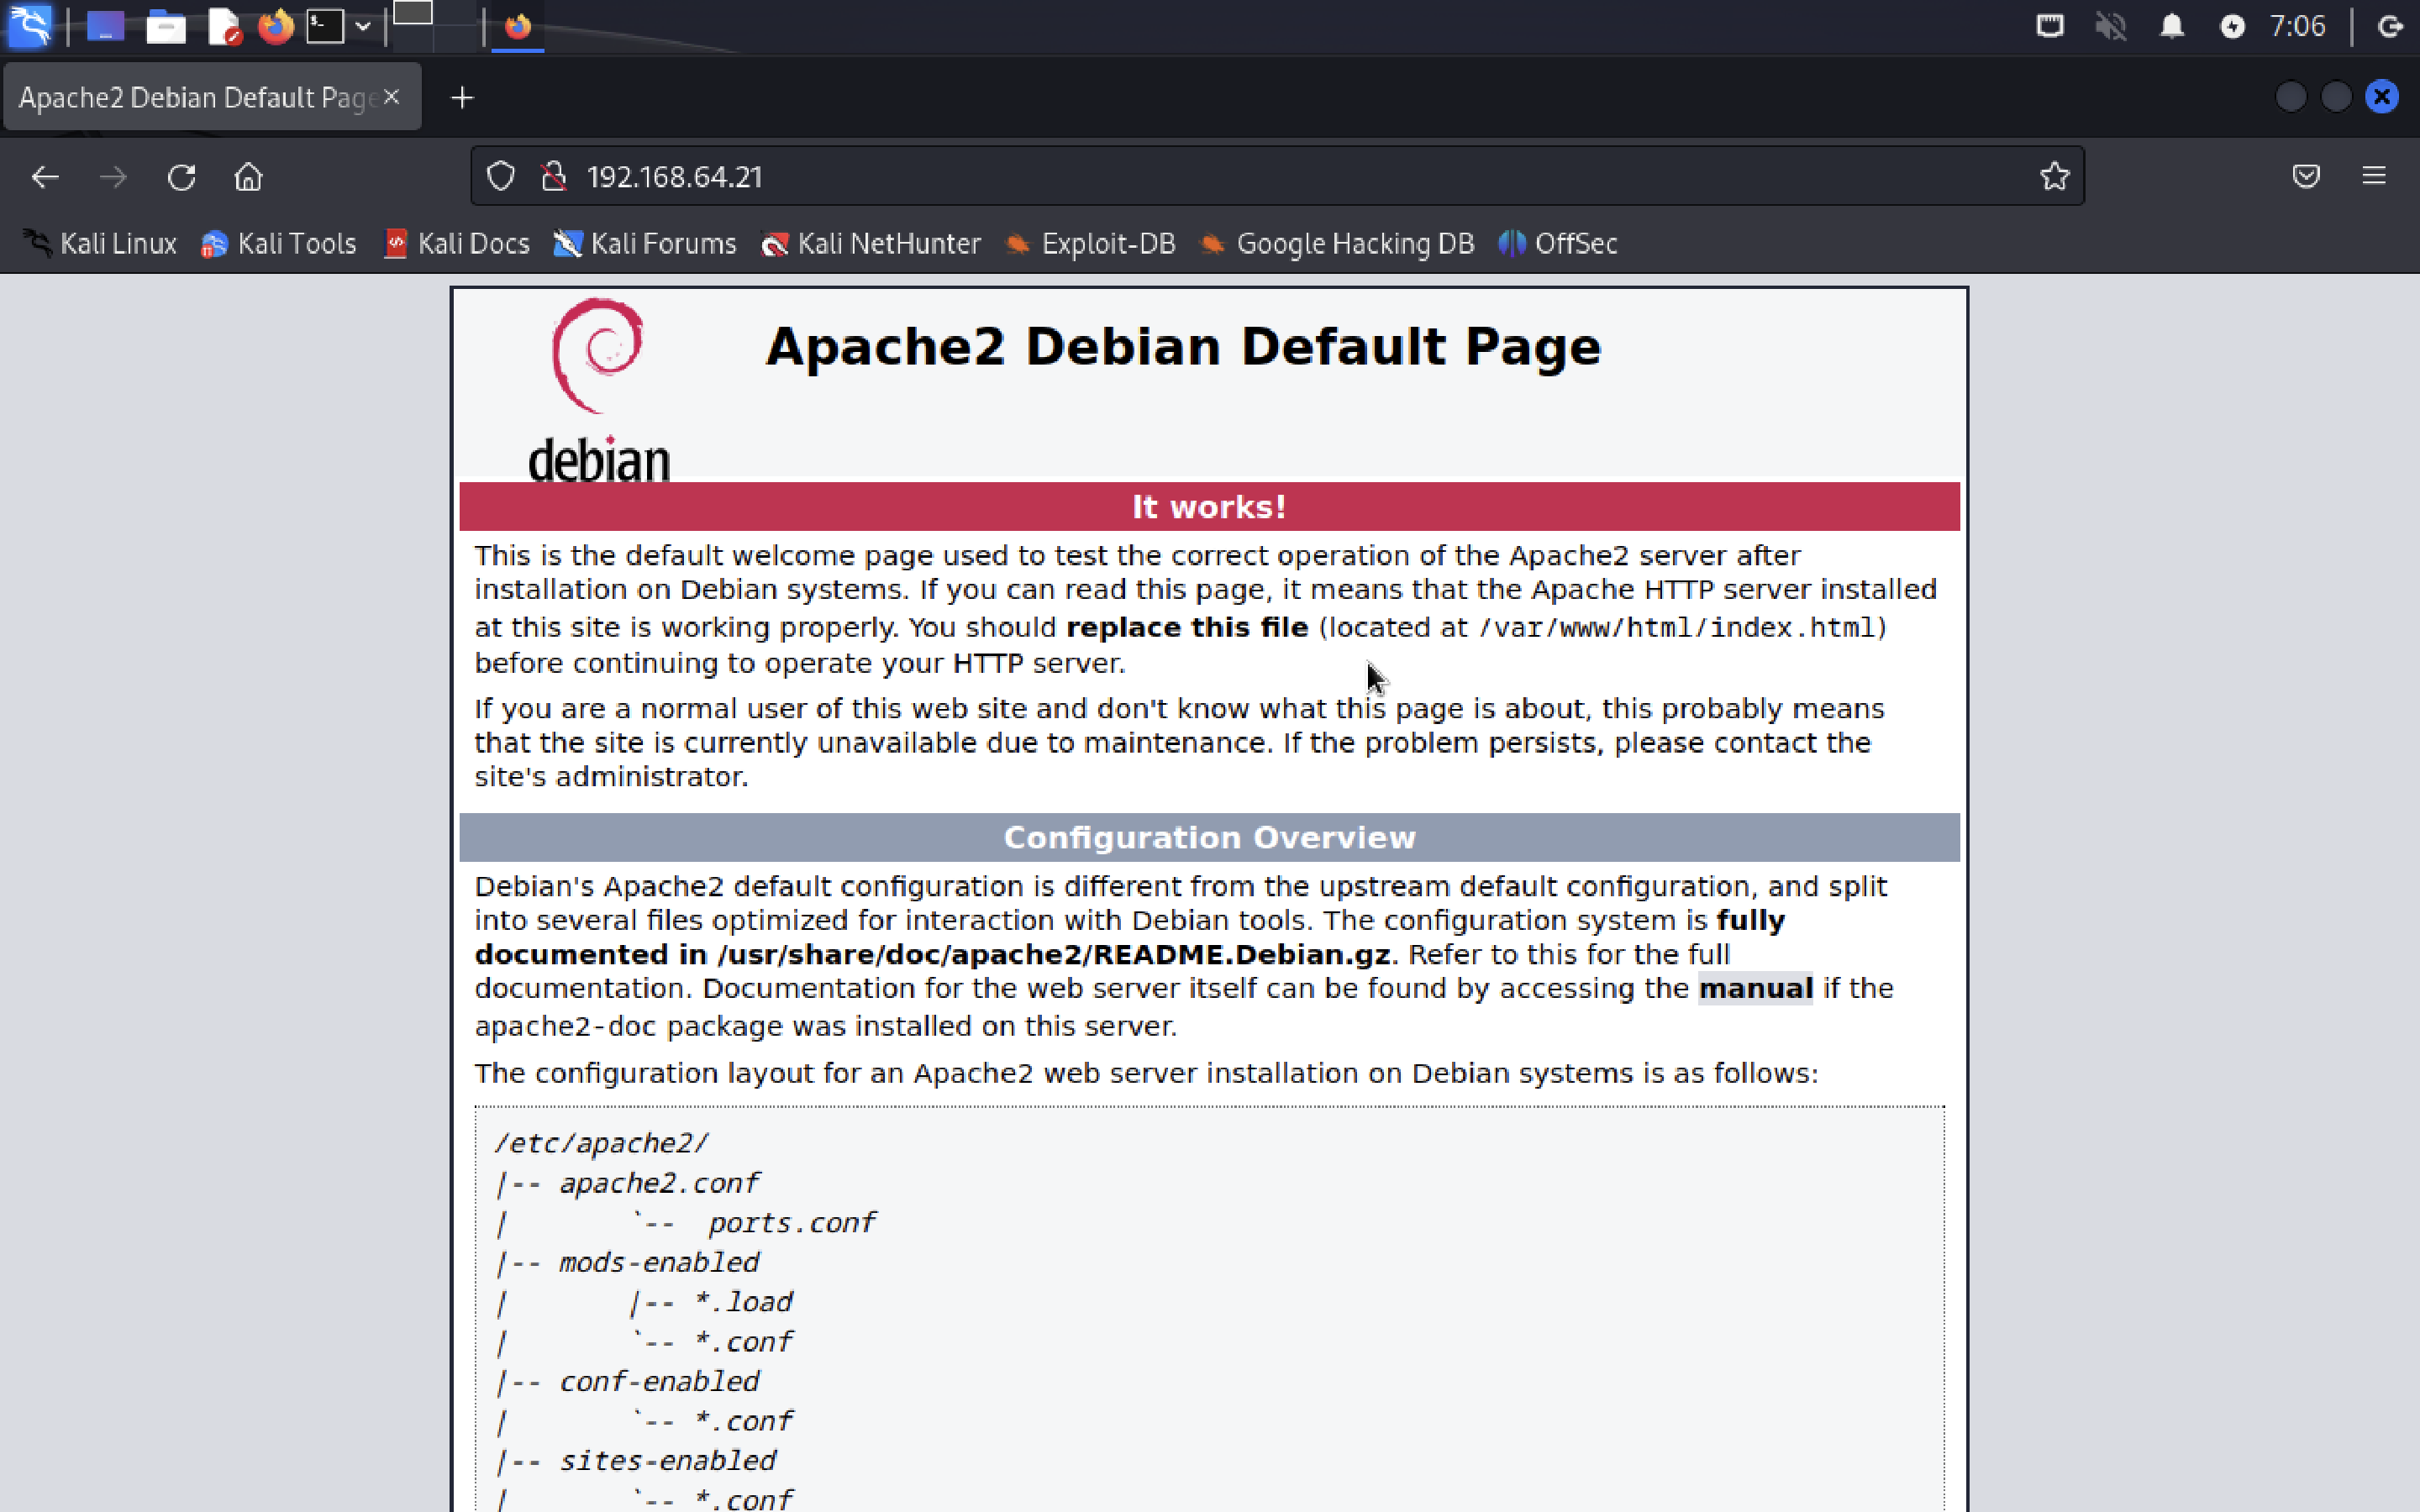
\includegraphics[width=\textwidth]{img/itworks.png}
    \caption{It actually works!}
\end{figure}

Come fase successiva dell'indagine, si è deciso di provvedere alla ricerca dei contenuti presenti sul server web in questione. Allo scopo, sarà utilizzato il tool \texttt{dirb}

\subsubsection{\texttt{dirb}}
\texttt{dirb} è probabilmente il web content scanner più diffuso. 
Come menzionato in precedenza, fa uso di un \textbf{dizionario} per interrogare il server web target ed identificare risorse basandosi sullo \textit{status code} della risposta HTTP. 
Le \textit{wordlists} che compongono il dizionario di questo tool sono presenti al percorso \texttt{/usr/share/wordlists/dirb/}.

Il tool viene invocato da riga di comando specificando come primo parametro la risorsa web da analizzare. È anche possibile salvare l'output del tool in un file mediante lo switch \texttt{-o}. 

Il report completo generato dal tool è disponibile nel file \texttt{noobbox-dirb.txt}, allegato al presente documento.

\begin{center}
    \texttt{dirb http://192.168.64.21/ -o noobbox-dirb.txt}
\end{center}

Facendo riferimento al report generato, salta subito all'occhio la presenza di una directory chiamata \texttt{wordpress/}. Con molta probabilità, quindi, il server web utilizza questo framework. Maggiori informazioni sul topic saranno fornite in una sezione \textit{ad hoc}.

Altre risorse presenti sul server sono di importanza relativamente bassa, in quanto fanno riferimento alla \textbf{documentazione} del server web in diverse lingue, presente nella directory \texttt{manual/}. Consultando questo endpoint è tuttavia possibile risalire alla versione del server web installato, ma quest'ultima è un'informazione già ottenuta utilizzando \texttt{nmap} nella fase precedente della target enumeration.

È inoltre presente una pagina denominata \texttt{server-status}, ma visitando quest'ultima si riceve lo \textit{status code} 403, che indica un \textbf{permesso negato}.


\begin{figure}[h!]
    \centering
    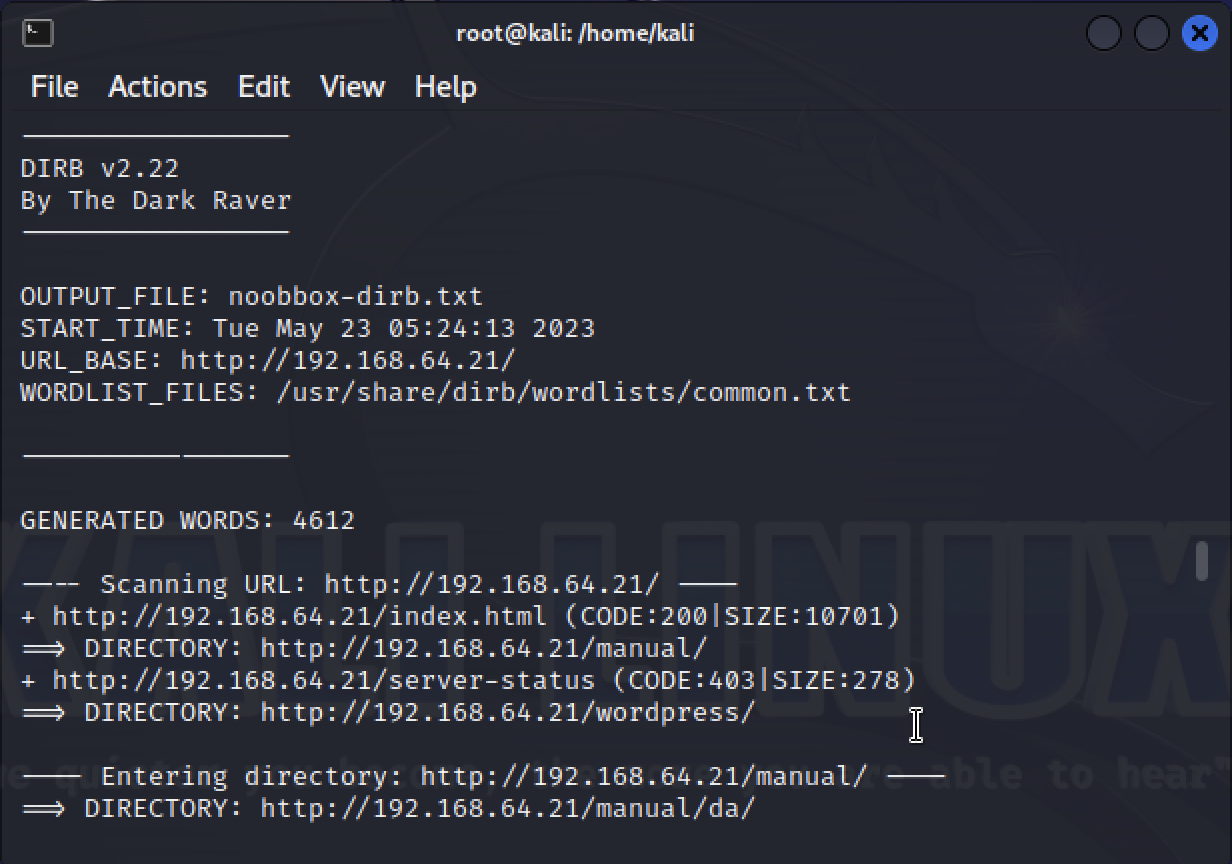
\includegraphics[width=\textwidth]{img/dirb-output.png}
    \caption{\texttt{dirb} ha rilevato una directory wordpress}
\end{figure}

\begin{figure}[h!]
    \centering
    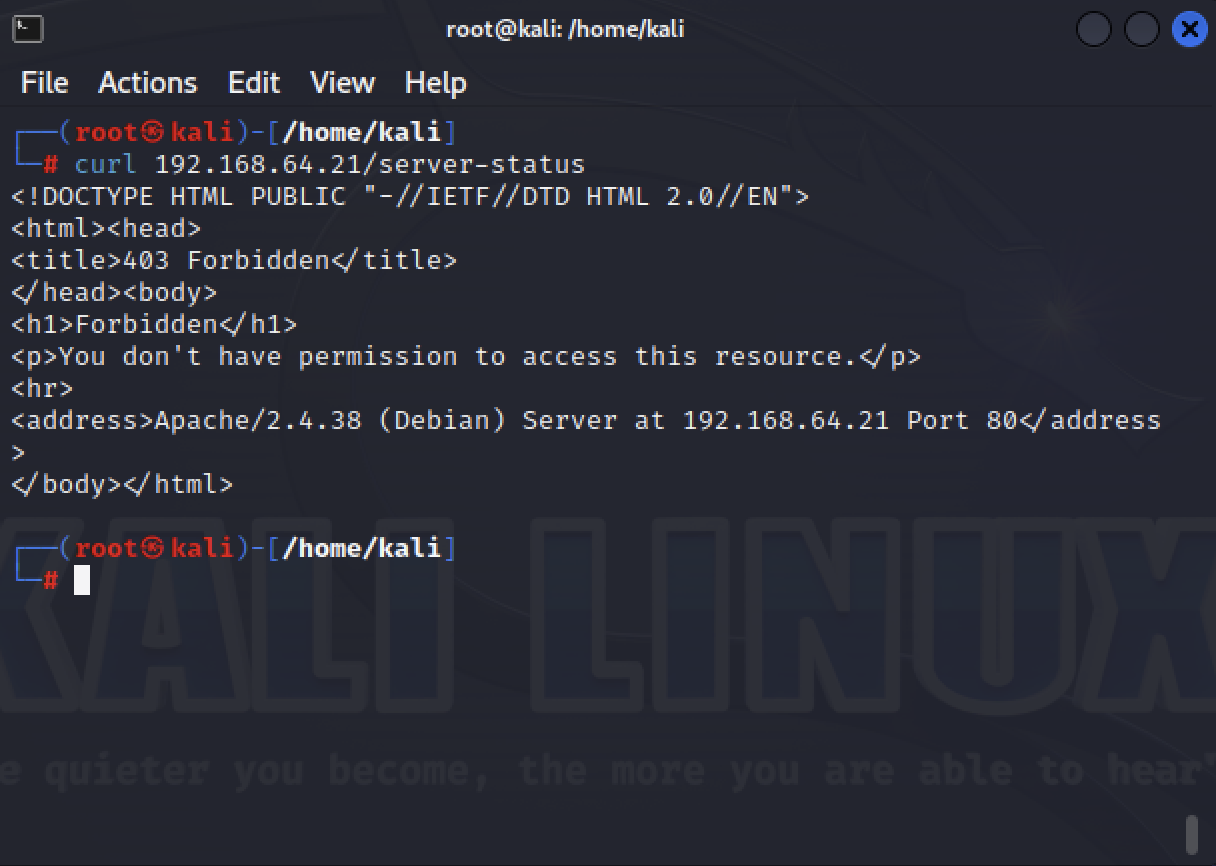
\includegraphics[width=\textwidth]{img/permission-denied.png}
    \caption{Ouch!}
\end{figure}

\newpage

Basandosi sull'output di \texttt{dirb} diventa subito evidente che il \textit{focus} dell'indagine debba cadere sull'analisi di una possibile installazione del framework \textbf{wordpress}.

È inoltre possibile configurare dirb per cercare file con determinate estensioni mediante lo switch \texttt{-X}. A questo scopo si è scelto di cercare immagini JPEG, file di testo in formato .txt, script PHP e documenti HTML nella root del web server.

Il comando diventa quindi:

\begin{center}
    \texttt{dirb http://192.168.64.21/ -X .jpg,.php,.txt,.html -o dirb-documents-output.txt}
\end{center}

Di seguito è presente l'output di questa scansione. Il report completo è allegato a questo documento nel file \texttt{dirb-documents-output.txt}.

\begin{figure}[h!]
    \centering
    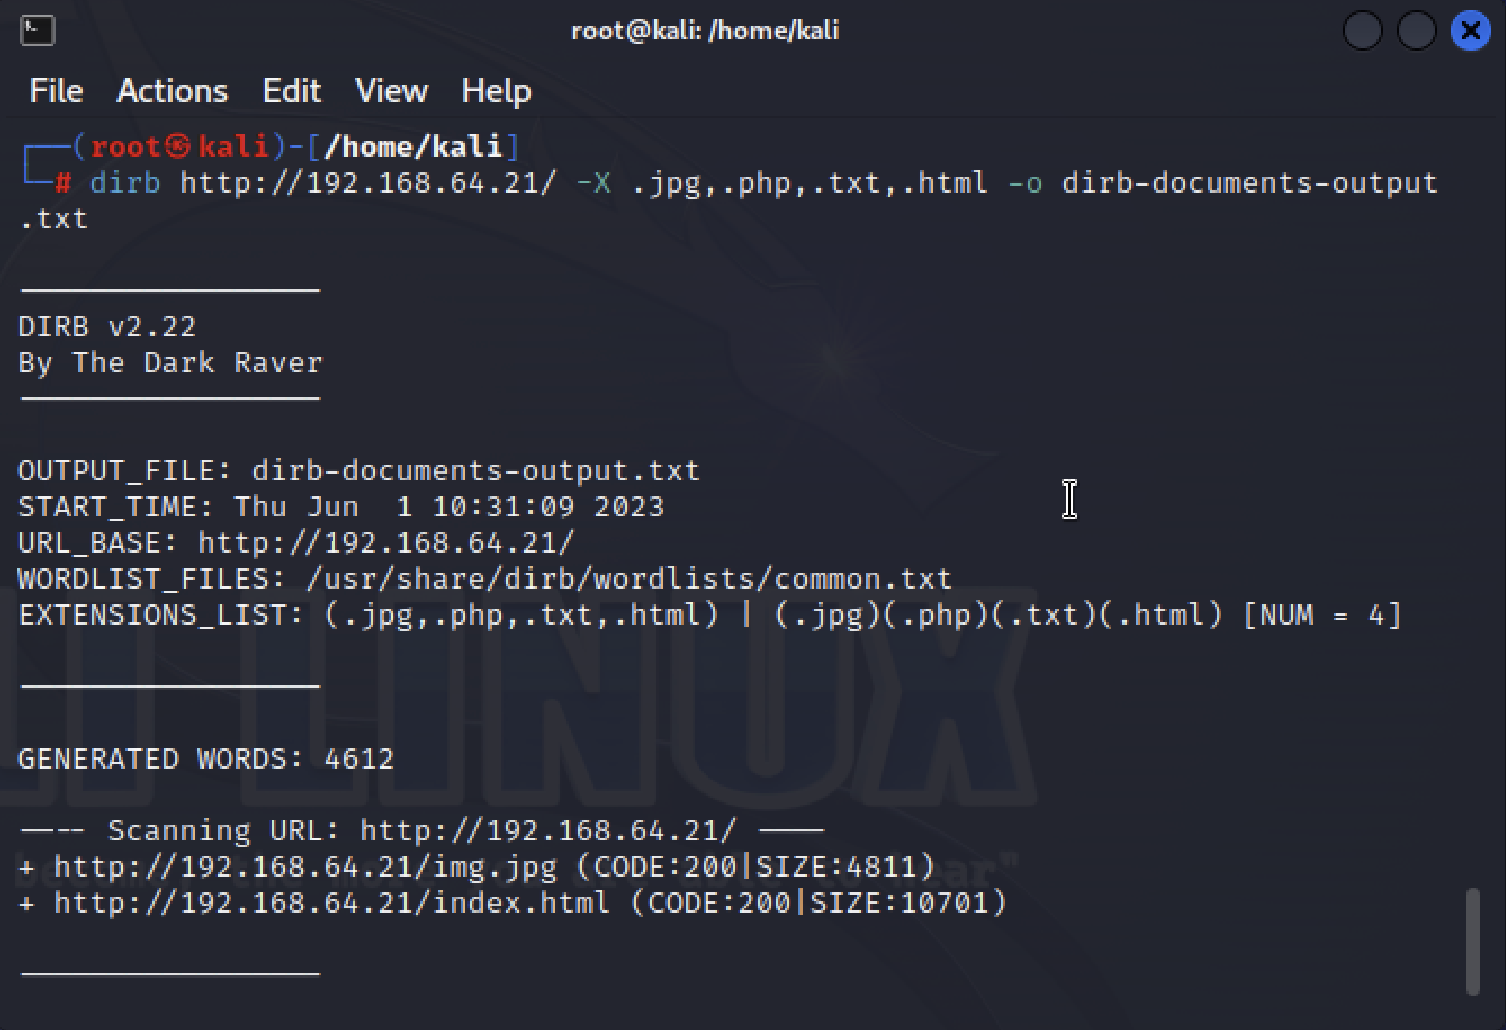
\includegraphics[width=\textwidth]{img/dirb-files-root.png}
    \caption{\texttt{dirb} ha trovato due file.}
\end{figure}

Come riportato in figura, è possibile notare la presenza di un file index.html, che contiene la pagina di default di Apache ma anche un file chiamato \texttt{img.jpg}. 

\begin{figure}[h!]
    \centering
    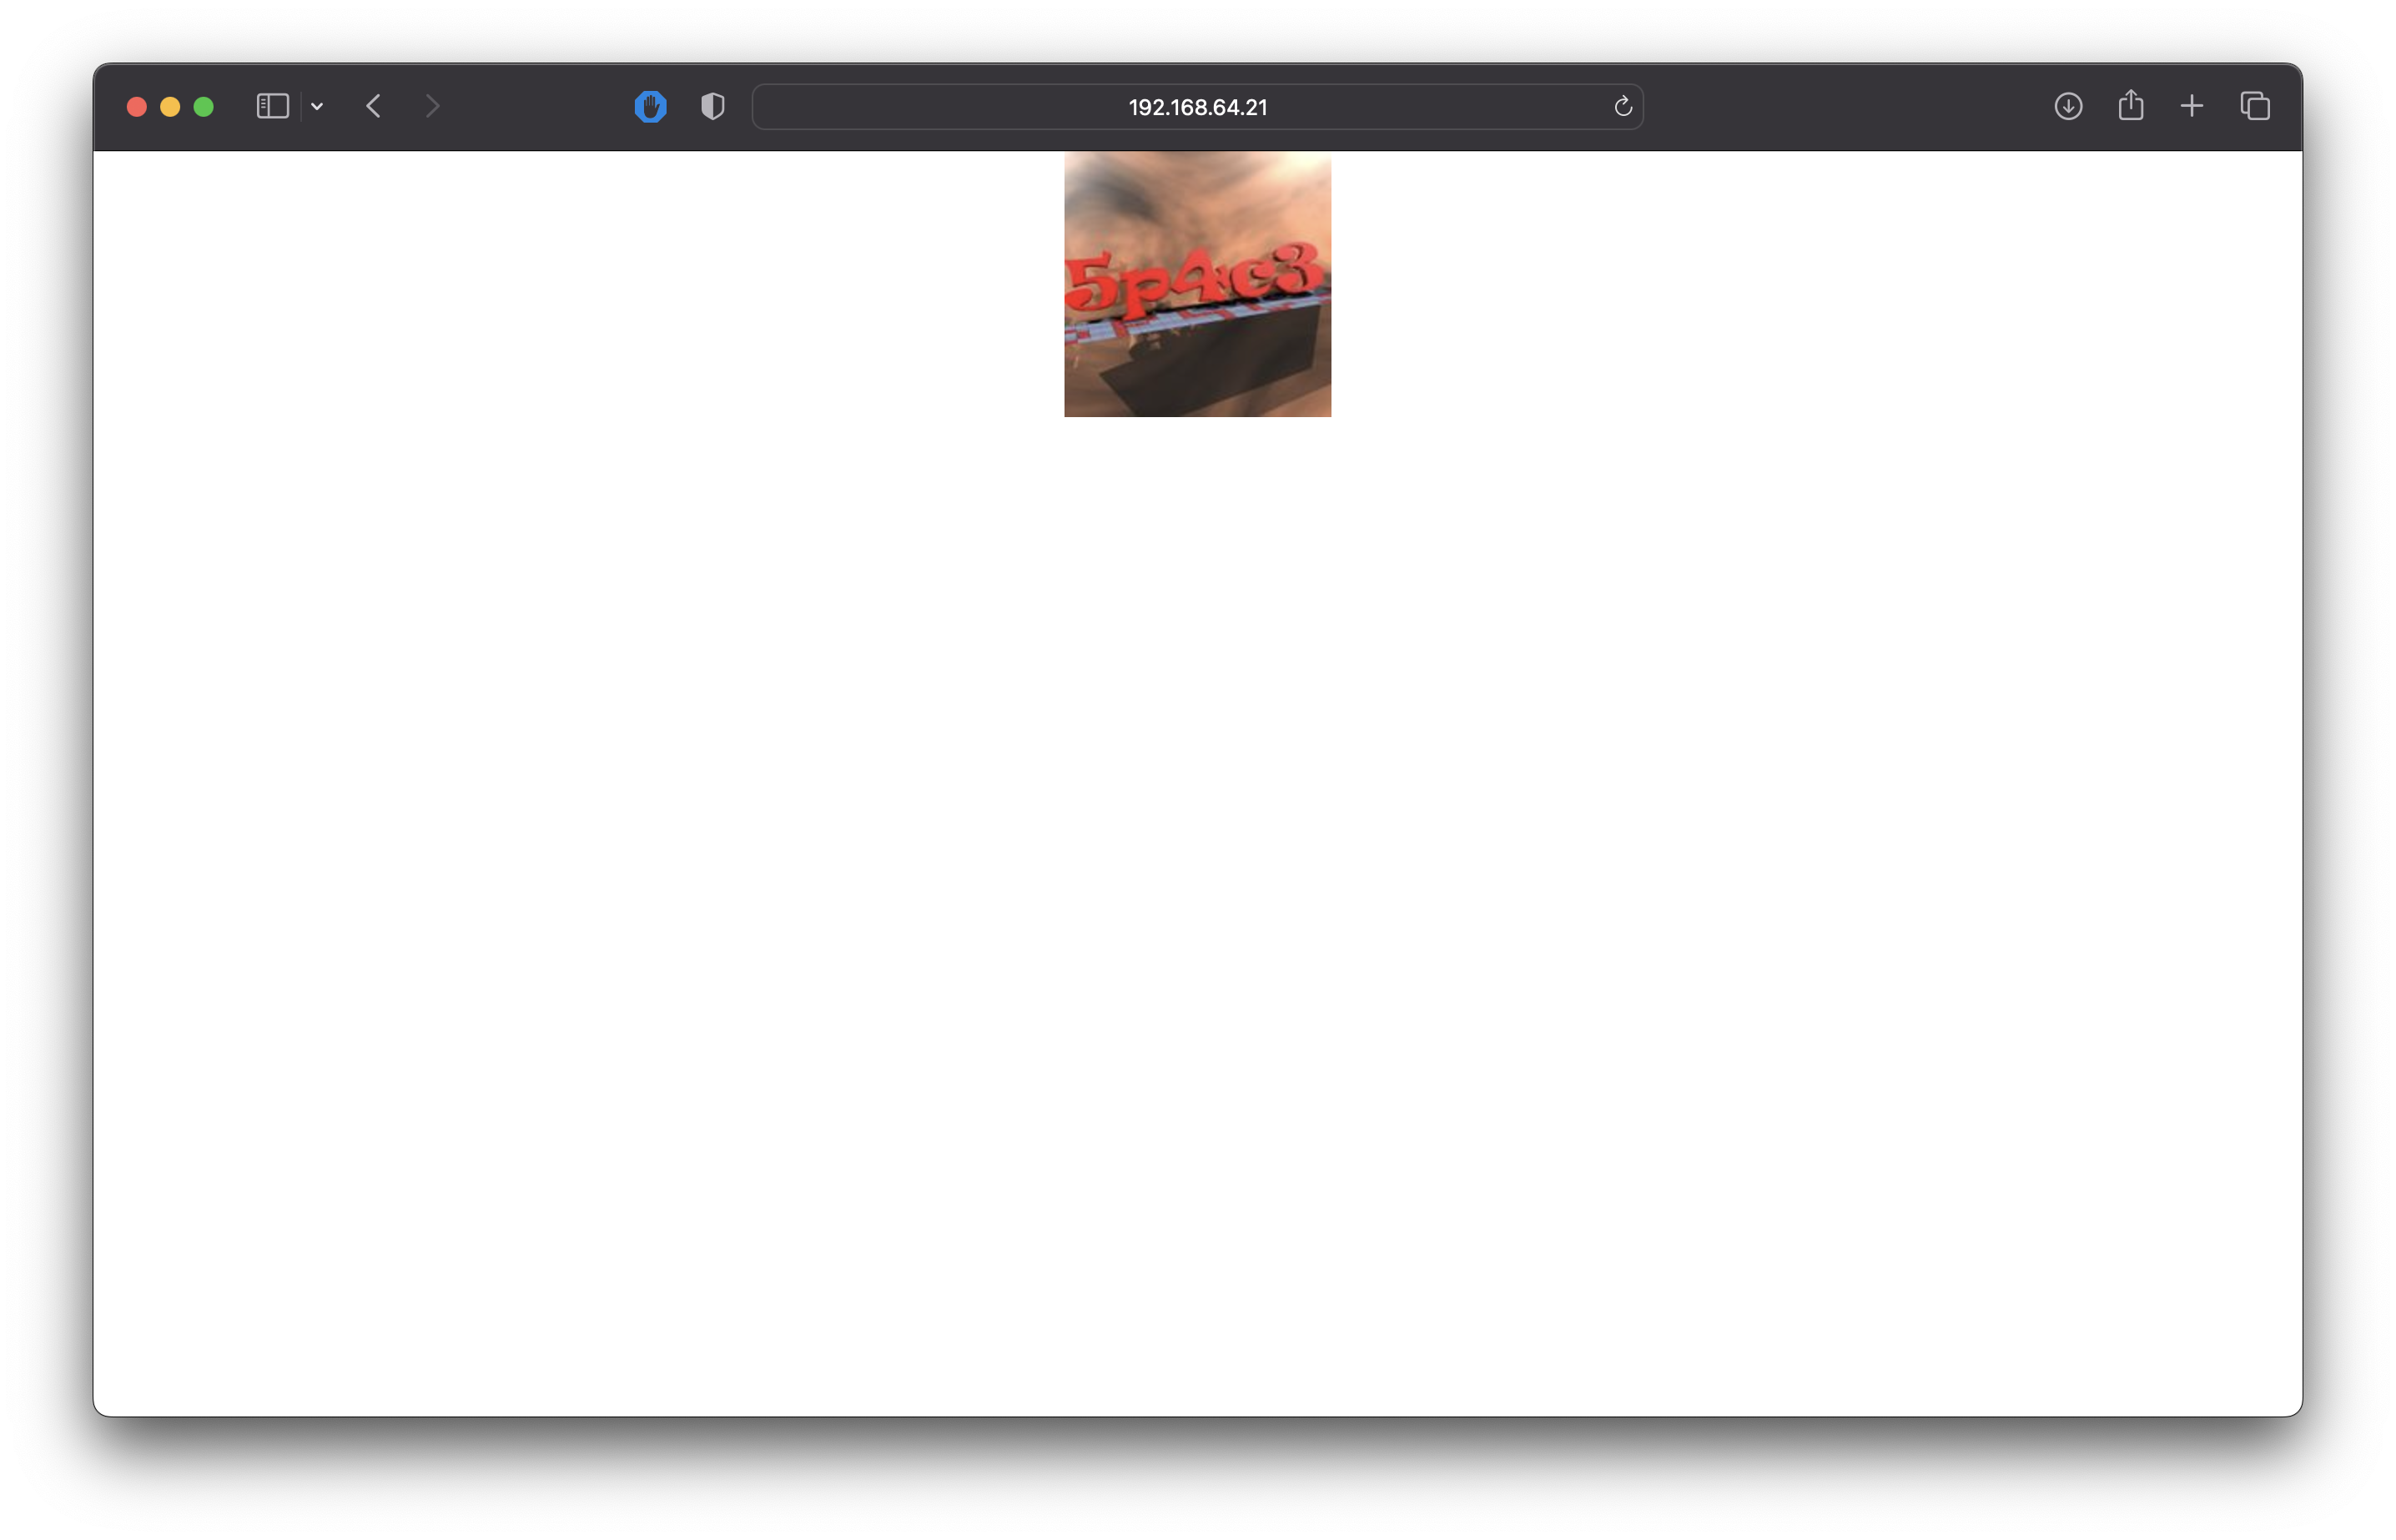
\includegraphics[width=\textwidth]{img/space.png}
    \caption{Space?}
\end{figure}

Aprendo il file visitando l'URL \texttt{192.168.64.21/img.jpg} si ottiene quanto mostrato nella Figura 12.

Si noti come nella seconda scansione (in cui sono state specificate le estensioni da considerare) non è avvenuta una ricerca ricorsiva. Per ovviare a questa problematica, verrà preso in considerazione il tool \texttt{feroxbuster}.

\subsubsection{\texttt{feroxbuster}}

\texttt{feroxbuster} può essere considerata un'alternativa al ben più noto tool \texttt{gobuster} e che risolve il suo difetto più grande: il mancato supporto alle scansioni ricorsive. \cite{feroxbuster}

Scritto nel linguaggio \textbf{Rust}, questo tool è presente nei repository di Kali Linux ed è installabile tramite il comando

\begin{center}
    \texttt{sudo apt-get install feroxbuster}
\end{center}

Eseguendo questo comando, verranno installati sia il tool che un apposito insieme di \textbf{wordlists}, presenti nel pacchetto \texttt{seclists}.

Il tool verrà usato per andare ad analizzare la cartella \texttt{/wordpress} per cercare di capire se il sito web offerto dalla macchina ne faccia effettivamente uso.

Il comando invocato a questo scopo è il seguente:

\begin{center}
    \texttt{feroxbuster -{}-url http://192.168.64.21/wordpress -{}-extensions php,jpg,txt,html -{}-output feroxbuster\_noobbox\_wordpress.txt  -{}-depth 10}
\end{center}

Data la prolissità dell'output, esso è stato salvato all'interno del file \texttt{feroxbuster\_noobbox\_wordpress.txt}, allegato al presente documento.

Consultando i risultati del tool, all'interno di tale cartella sembra sia \textbf{sia effettivamente presente un'installazione di Wordpress}. Visitando l'endpoint \texttt{wordpress/} si ottiene invece quanto mostrato in Figura 14.

\begin{figure}[h!]
    \centering
    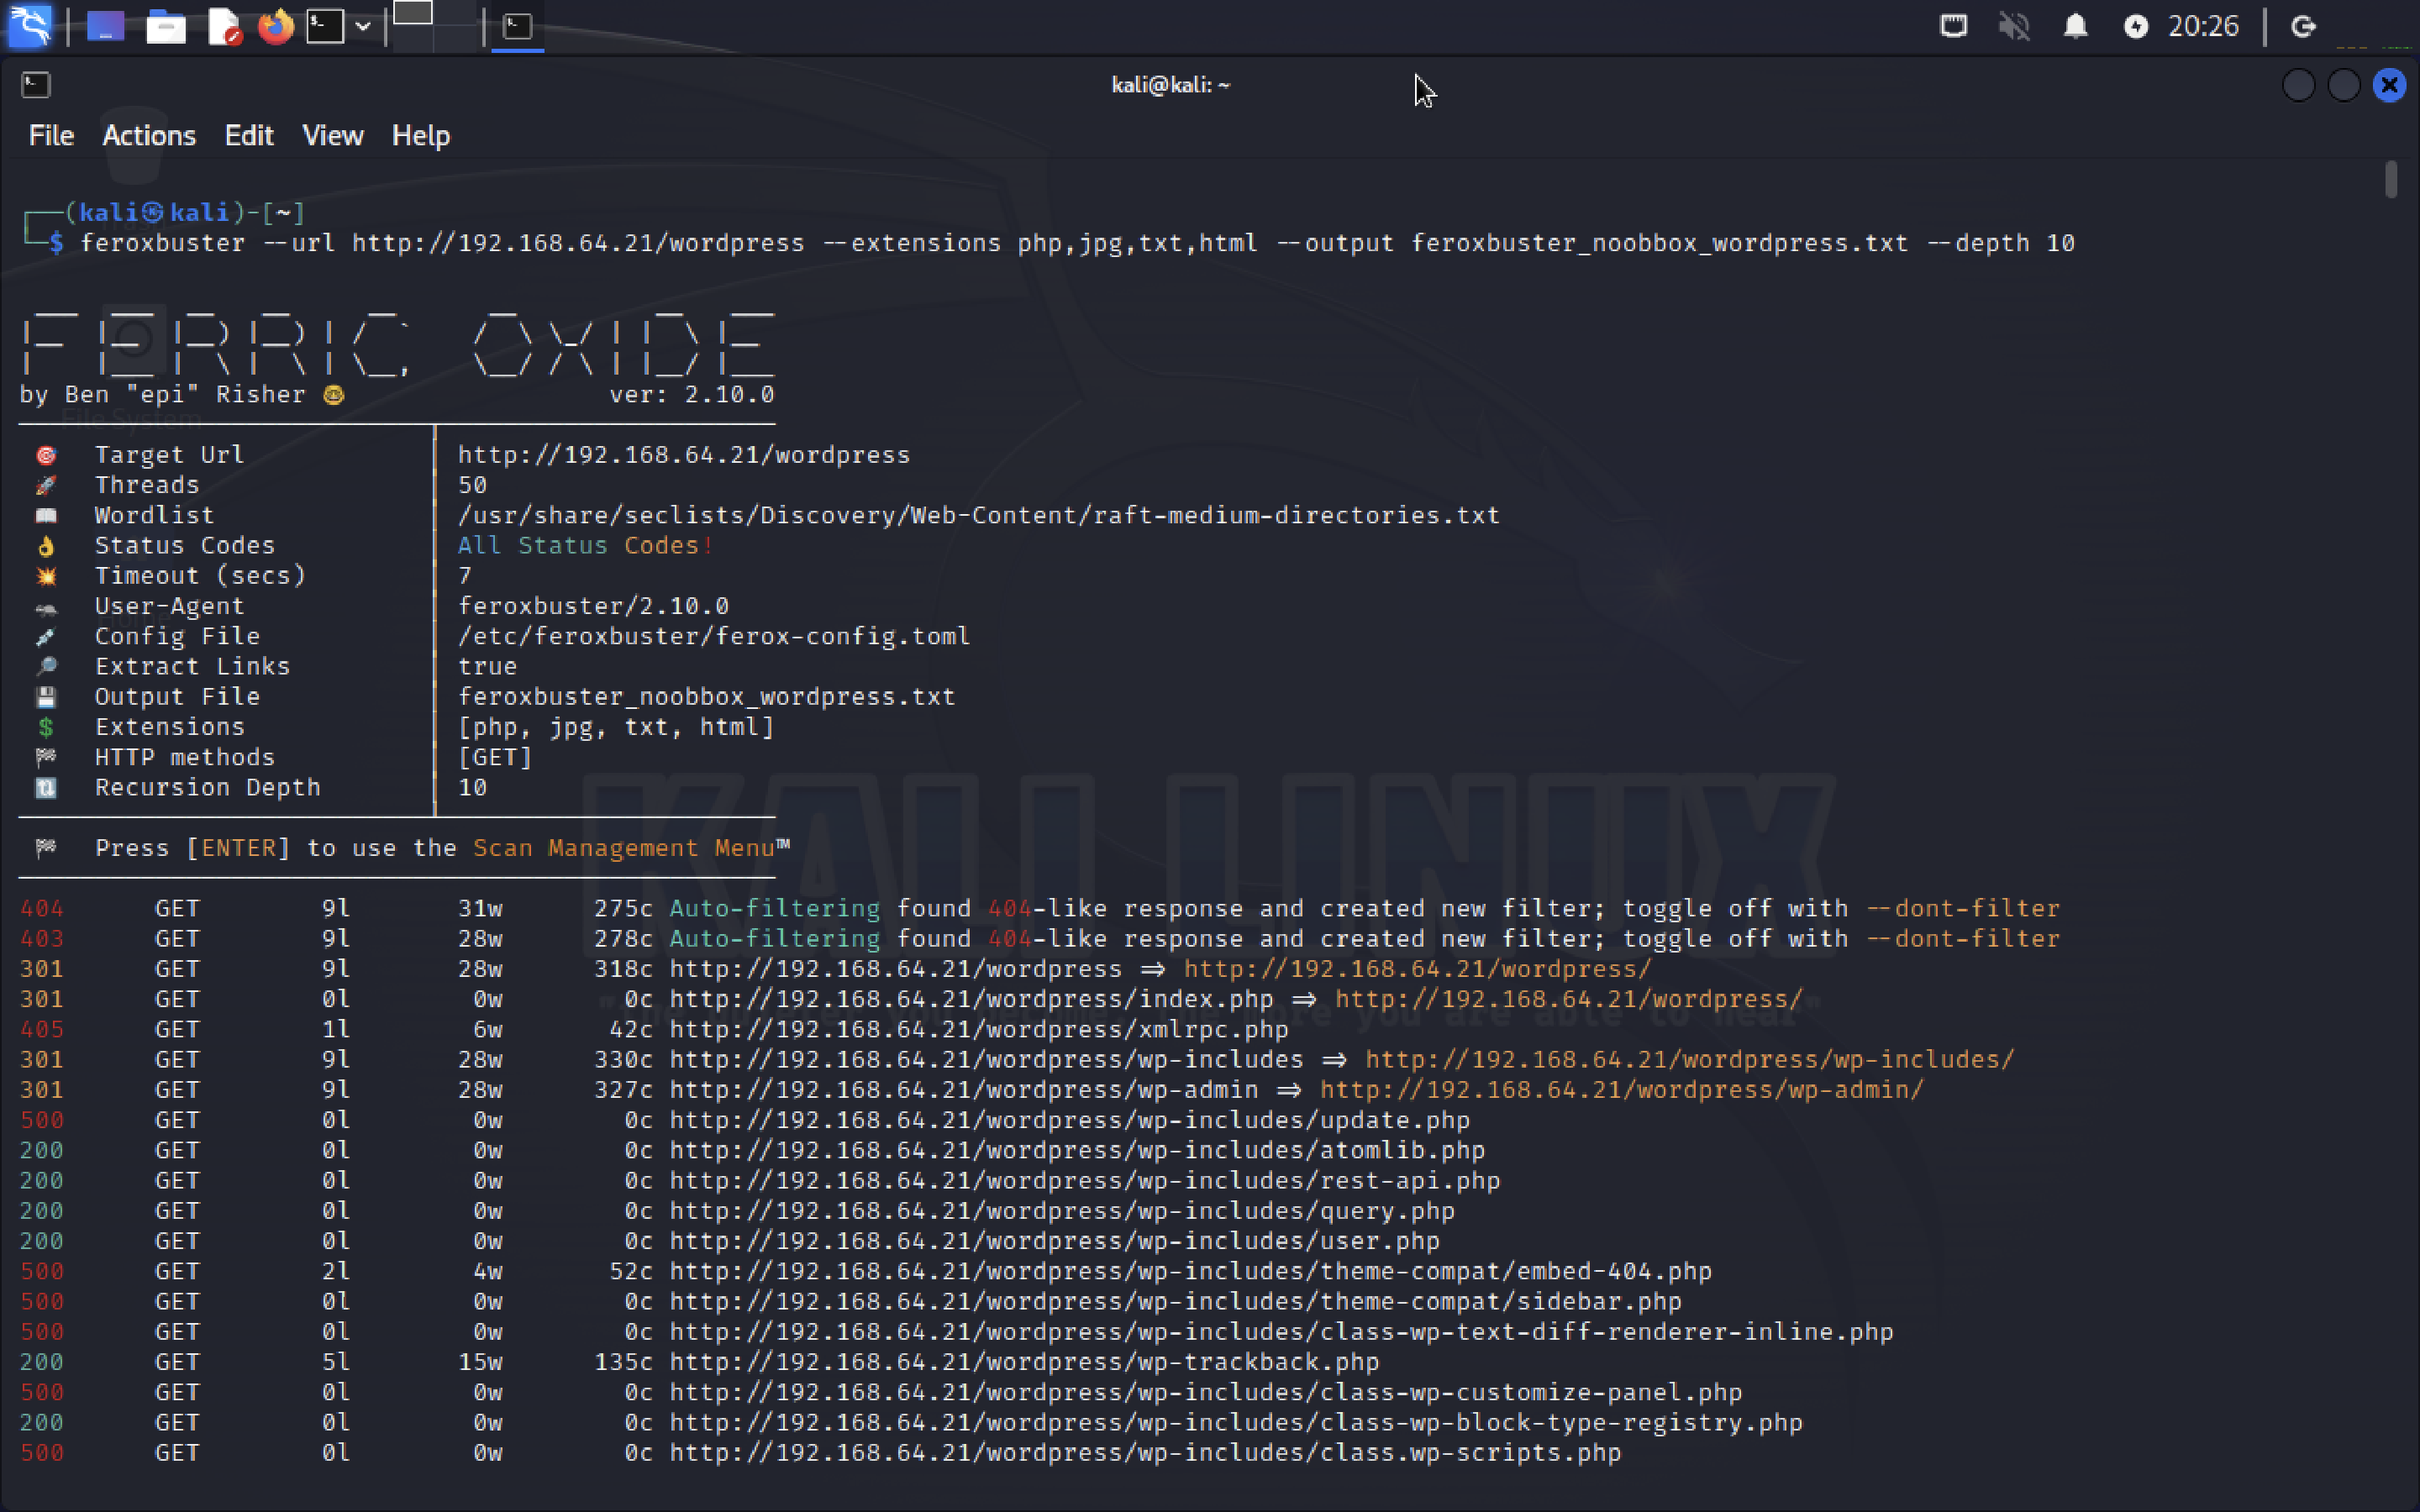
\includegraphics[width=\textwidth]{img/feroxbuster.png}
    \caption{\texttt{feroxbuster} in esecuzione}
\end{figure}

\begin{figure}[h!]
    \centering
    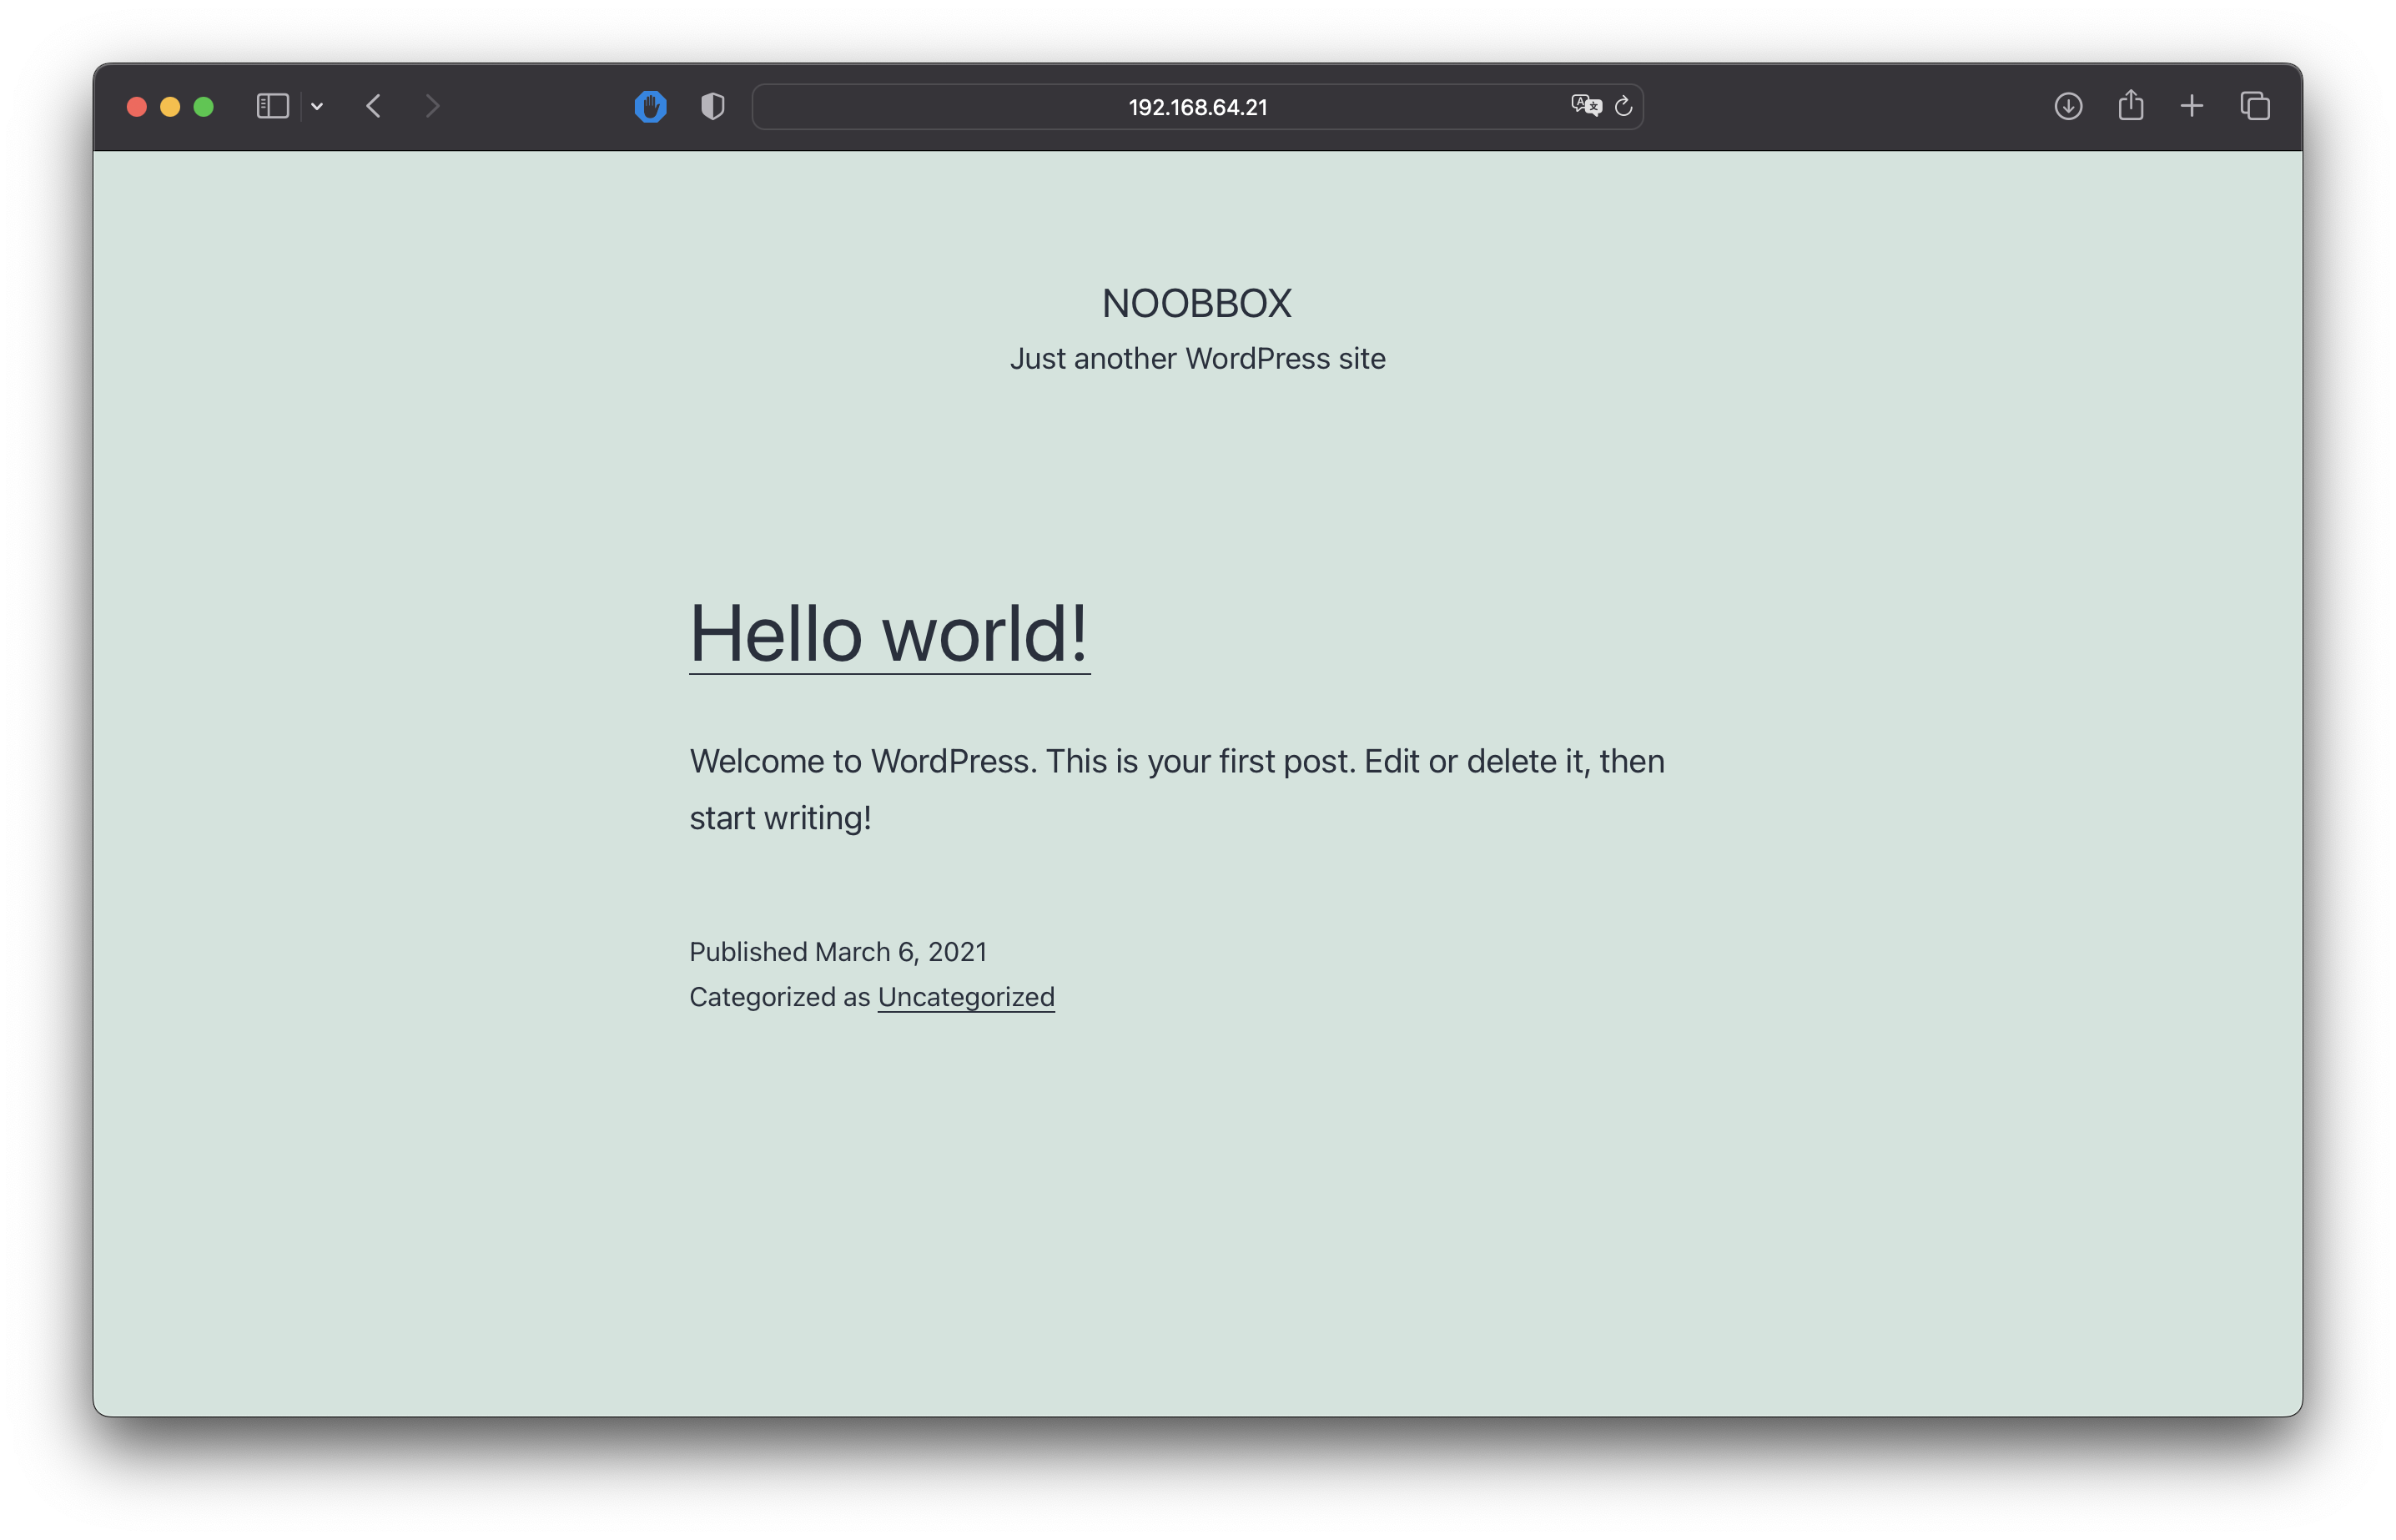
\includegraphics[width=\textwidth]{img/wordpress.png}
    \caption{"Just another WordPress site"}
\end{figure}

\newpage
\newpage
\newpage

\subsubsection{Wordpress ai raggi X: \texttt{wpscan}}

Avendo appurato che sul server web sia in esecuzione un'istanza di \textbf{wordpress}, è possibile proseguire con il processo di enumerazione iniziato in precedenza utilizzando il tool \texttt{wpscan}, che permette un'enumerazione mirata dell'istanza di tale framework in esecuzione sull'asset in analisi.

In questa fase dell'analisi, viene utilizzato il tool nella sua configurazione di default con l'aggiunta di un processo di enumerazione degli \textbf{utenti} (switch \texttt{-e u}). Si è deciso di concentrarsi su questo aspetto poiché in precedenza era stata rinvenuta un'immagine che si assume possa essere una \textbf{password}. Avere a disposizione una tale coppia di credenziali permette non solo di accedere al \textbf{pannello di amministrazione} ma anche, mediante il tool \textbf{Metasploit}, ad una \textbf{shell} sulla macchina su cui Wordpress è in esecuzione.

Ulteriori informazioni su questo aspetto saranno forniti nelle sezioni successive.

In ogni caso, il comando utilizzato è il seguente:

\begin{center}
    \texttt{wpscan -{}-url 192.168.64.21/wordpress/ -e u}
\end{center}

Il risultato dell'esecuzione del tool è allegato al presente documento, ma in sostanza è stato determinato che:

\begin{itemize}
    \item La versione del framework risulta essere la 6.2.2, rilasciata il 20 maggio 2023; \footnote{Si tenga presente che Wordpress implementa un meccanismo di aggiornamento automatico del framework, attivo di default su tutti i siti web. \cite{wordpress-autoupdate}}
    \item È stato identificato l'utente \textbf{noobbox}; 
\end{itemize}

\begin{figure}[h!]
    \centering
    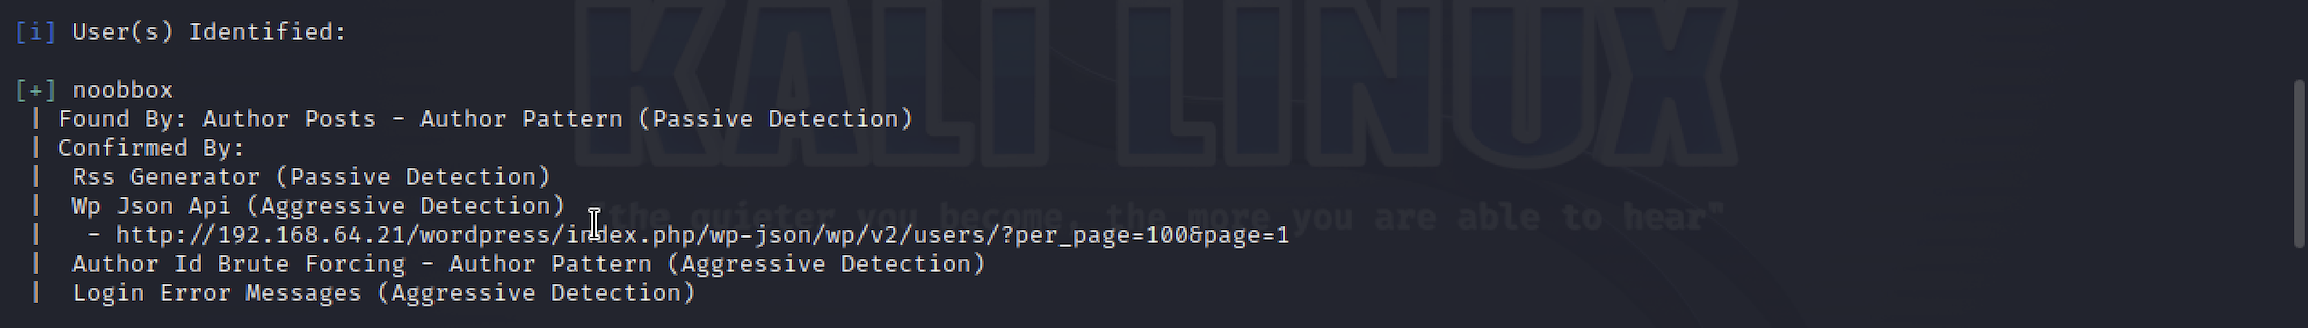
\includegraphics[width=\textwidth]{img/wpscan_user.png}
    \caption{\texttt{wpscan} ha rilevato un utente}
\end{figure}

Una successiva analisi volta alla ricerca di \textit{plug-ins} in uso da questa istanza del framework (mediante lo switch \texttt{-e p}) ha invece dato esito \textbf{negativo} e quindi non viene mostrata.

\newpage
\section{Vulnerability Mapping}
Le informazioni ottenute nella fase di Target Enumeration permettono già di definire una direzione chiara per la fase di \textbf{Exploitation}. In questa fase verrà invece descritta la strategia per identificare e riportare tutte le vulnerabilità presenti sull'asset usando i tools \textbf{OpenVAS} e \textbf{Nessus}.

\subsection{OpenVAS}
\textbf{OpenVAS} (\textit{Open Vulnerability Assessment Scanner}) è un tool open source messo a disposizione dall'azienda \textbf{Greenborne} che permette l'analisi automatica di asset, in maniera autenticata e non autenticata.\cite{openvas}

Questo tool è installabile direttamente dai repository di Kali Linux mediante il comando:

\begin{center}
    \texttt{sudo apt-get install openvas}
\end{center}

che permette il downlaod del tool insieme alle sue dipendenze. Si configura mediante lo script \texttt{gvm-setup} e si avvia mediante lo script \texttt{gvm-start} che si occuperà di avviare tutti i servizi e di mettere a disposizione un'interfaccia web all'indirizzo \texttt{localhost:9392}.

\begin{figure}[h!]
    \centering
    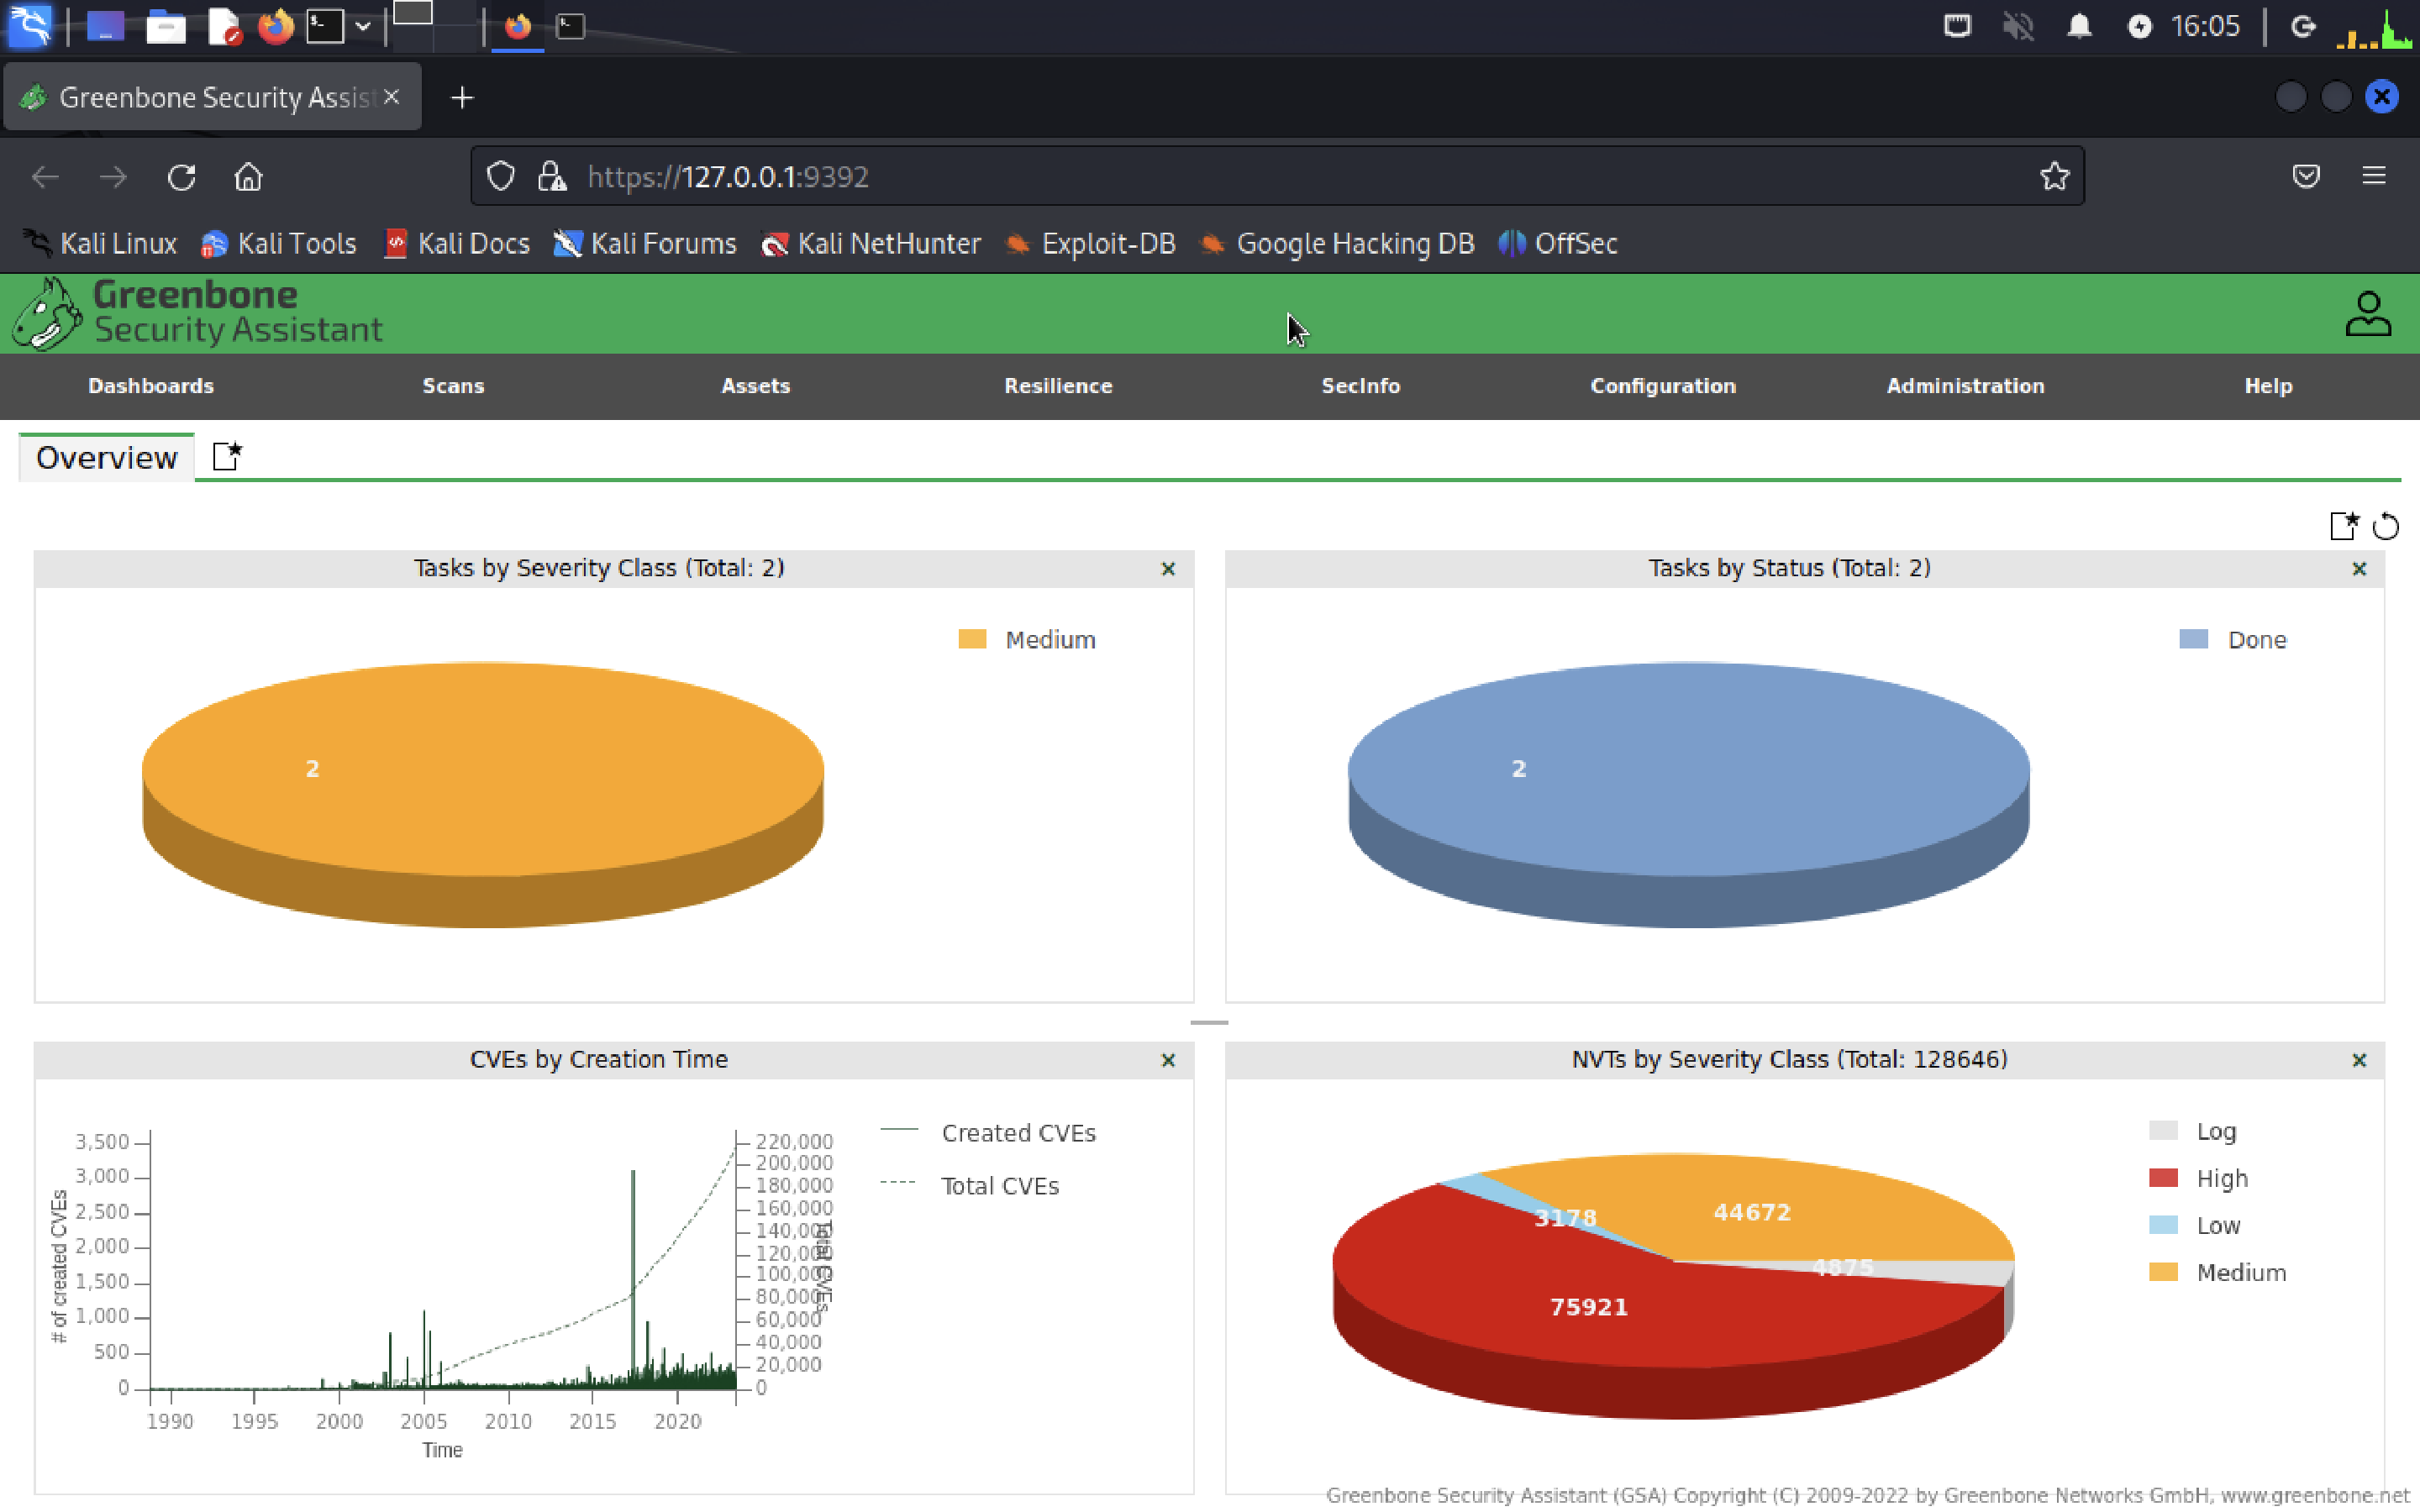
\includegraphics[width=0.8 \textwidth]{img/openvas-dashboard.png}
    \caption{La \textit{dashboard} di OpenVAS}
\end{figure}

Questo tool è stato utilizzato nella sua configurazione \textbf{\textit{Full and Fast}}, che permette un'analisi completa dell'asset. Nella Figura 17 viene mostrata l'interfaccia di creazione di un nuovo task di scansione.

\begin{figure}[h!]
    \centering
    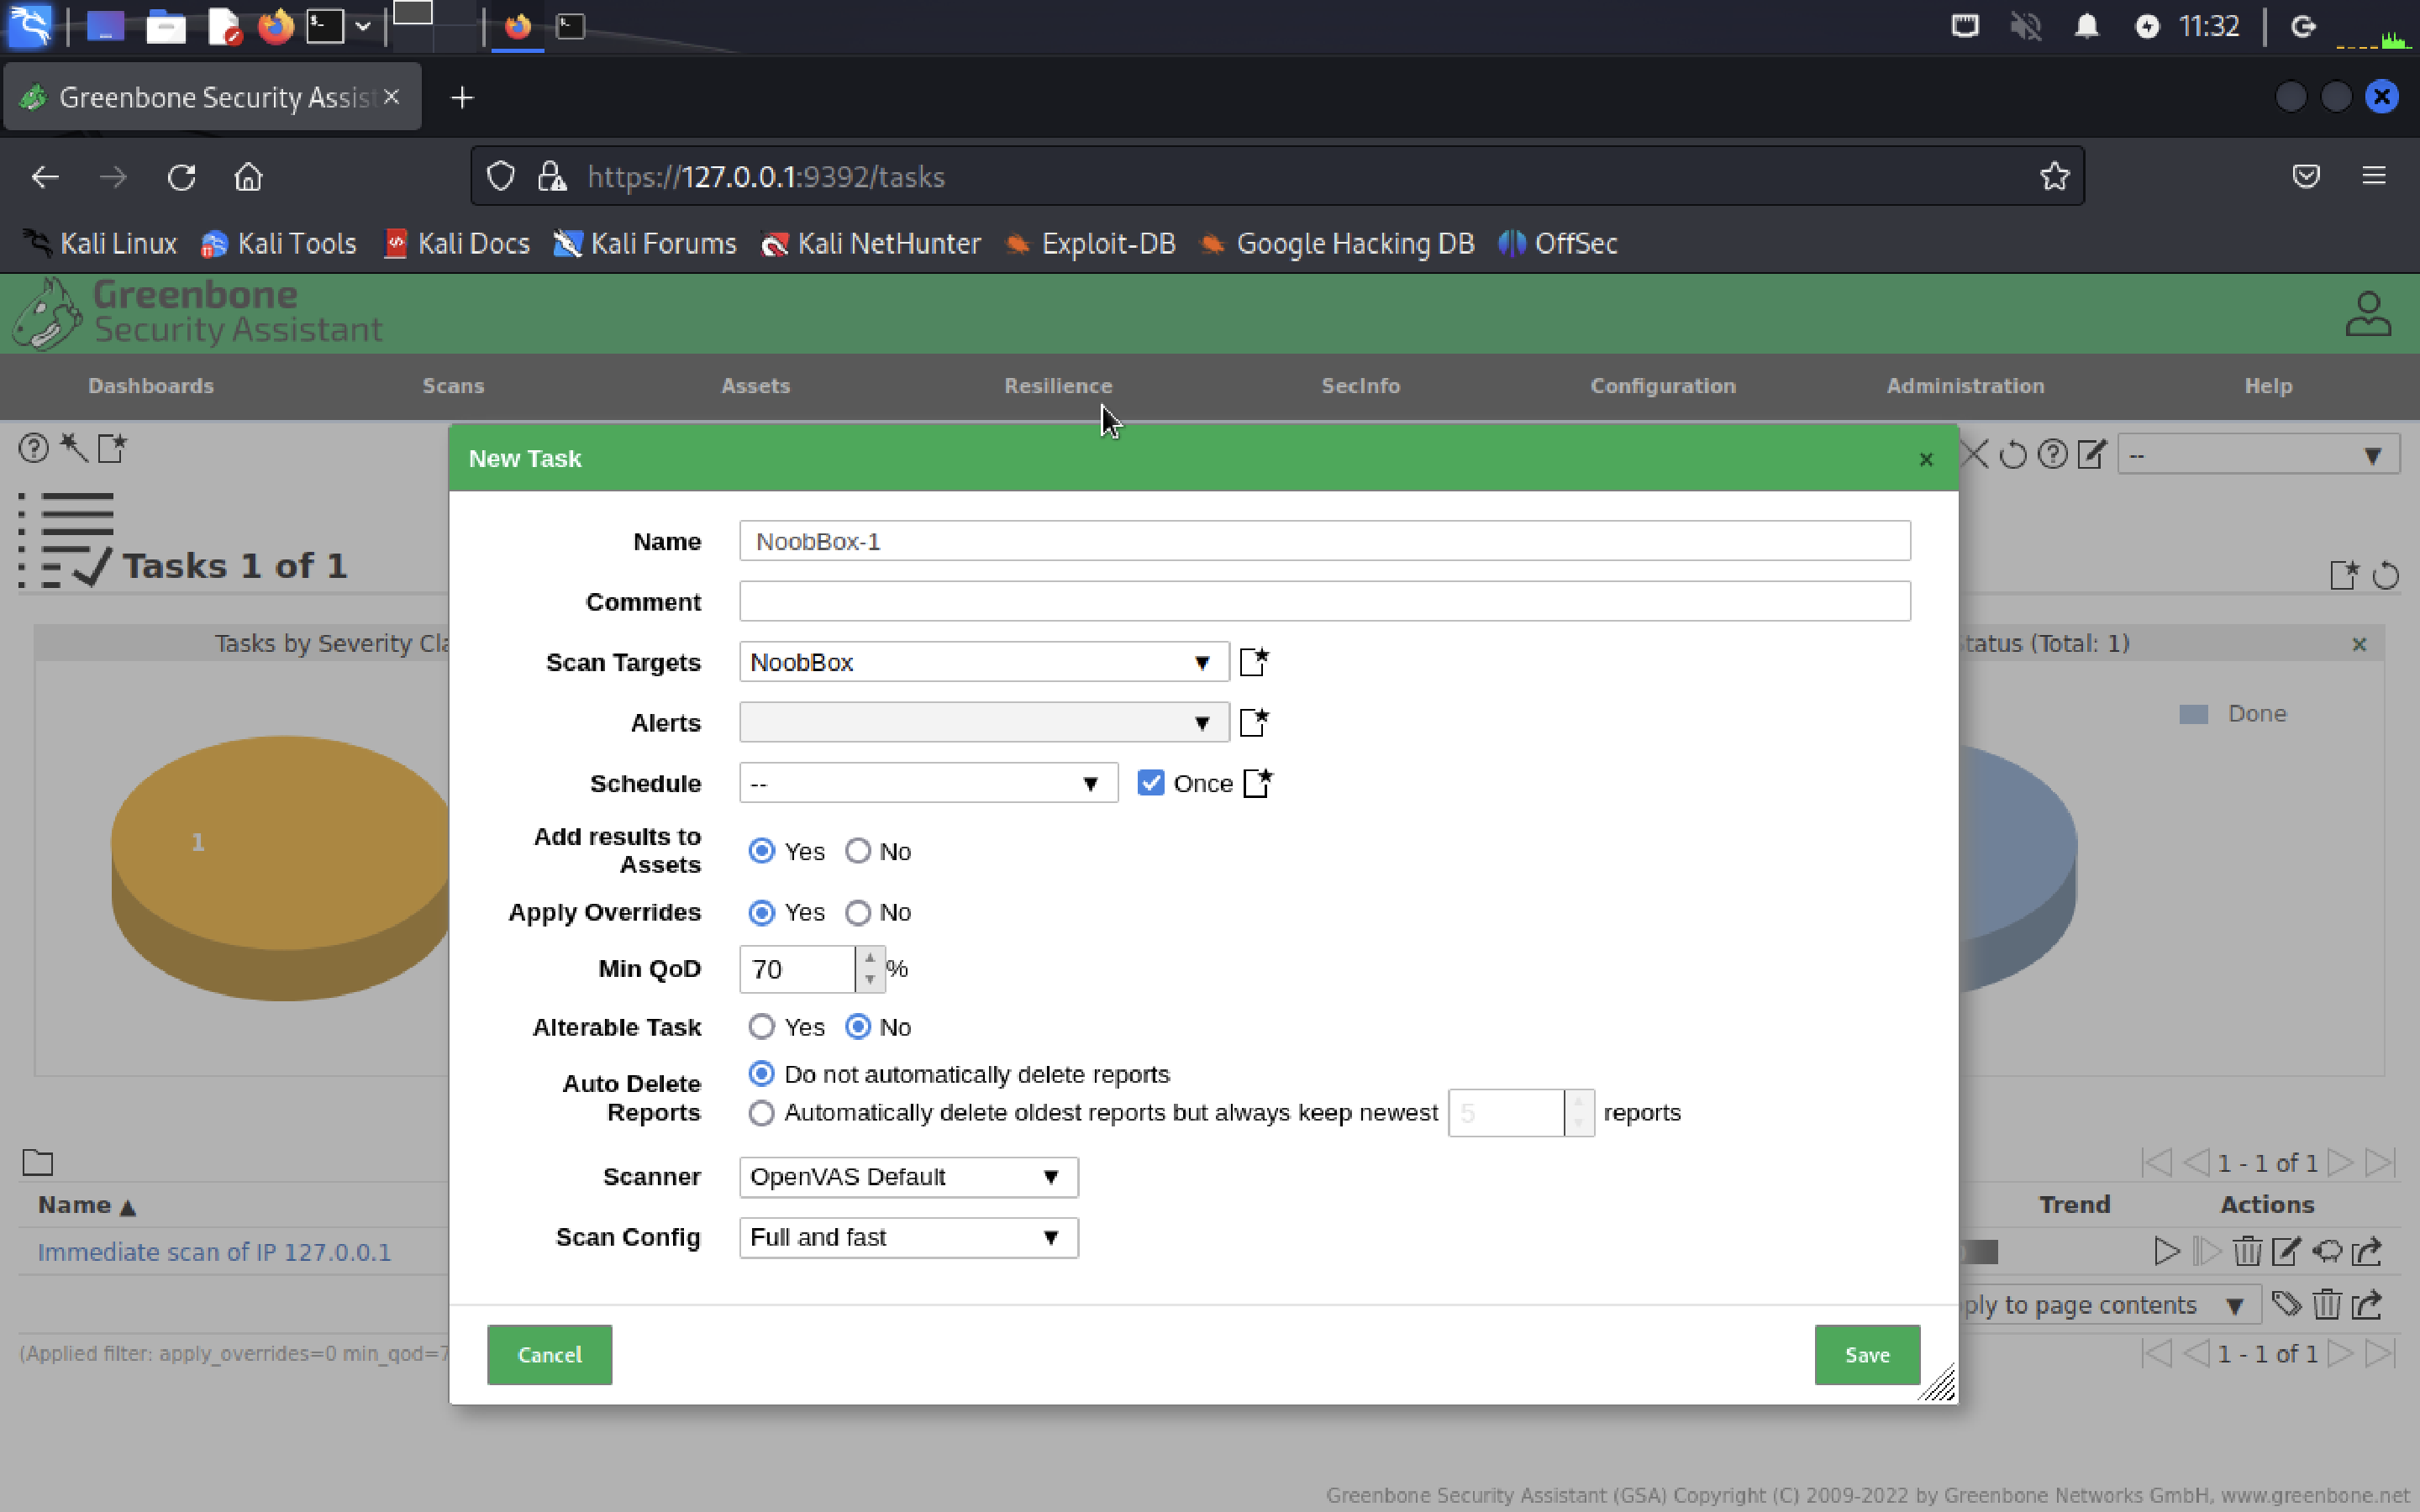
\includegraphics[width=\textwidth]{img/openvas-scan-task.png}
    \caption{Nuovo task}
\end{figure}

\subsubsection{OpenVAS: i risultati}
I risultati riportati dal tool dopo la scansione sono già filtrati e vengono considerate le vulnerabilità che hanno il valore di \textbf{QoD} (\textit{Quality of Detection}) pari o maggiore al \textbf{70\%}.

\begin{figure}[h!]
    \centering
    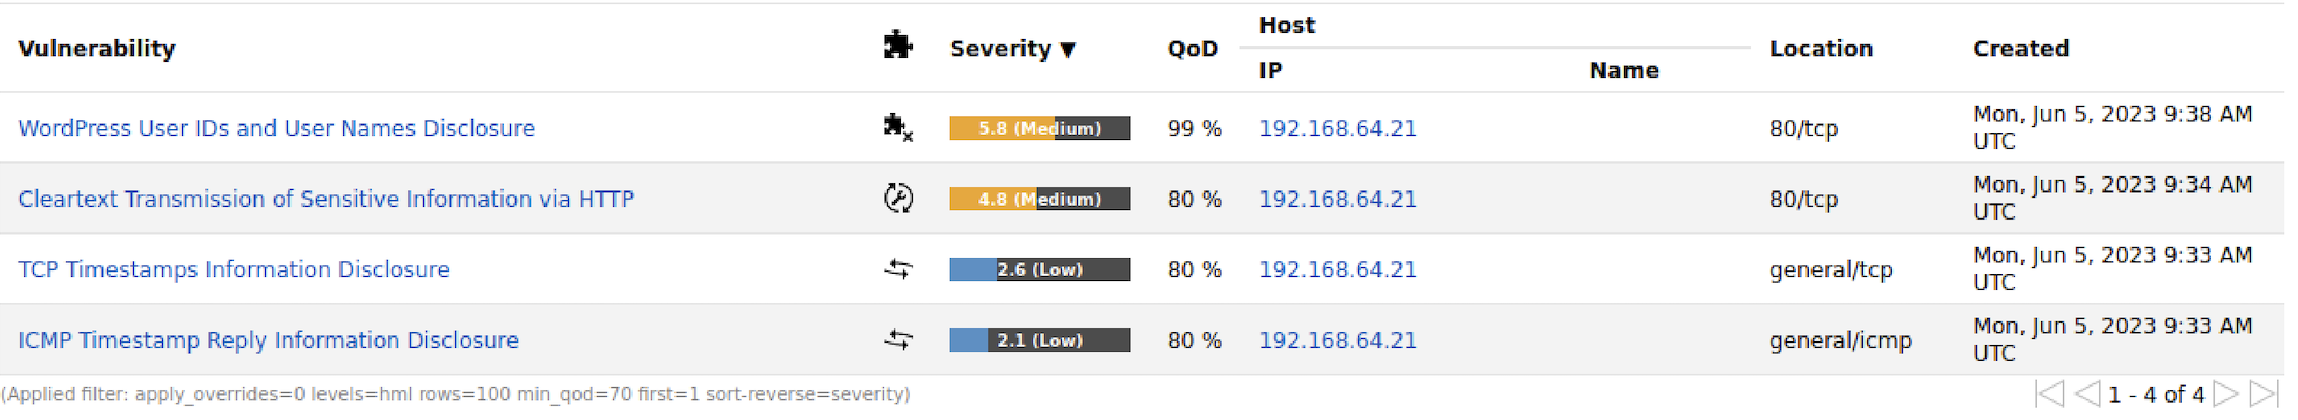
\includegraphics[width=\textwidth]{img/openvas-results.png}
    \caption{I risultati della scansione}
\end{figure}


Una discussione dettagliata sui risultati dei tool viene affrontata in una sezione apposita nel \textbf{Penetration Testing Report}, consegnato insieme al presente documento, ma in linea di massima le informazioni più importanti ottenute riguardano:

\begin{itemize}
    \item Non è presente alcun tipo di cifratura delle informazioni in transito da e verso il server;
    \item È stato possibile \textbf{enumerare gli utenti di Wordpress}, ad ulteriore conferma di quanto riscontrato in precedenza utilizzando \texttt{wpscan}.
\end{itemize}

\subsection{Nessus}
Il secondo tool utilizzato nella fase di Vulnerability Mapping consiste in \textbf{Nessus}, tool fornito dall'azienda \textbf{Tenable} che mette a disposizione sia una versione gratuita (denominata \textbf{Nessus Essentials}) che una versione a pagamento pensata per gli utenti Enterprise. Allo scopo di questa analisi viene utilizzata la versione Essentials.

\subsubsection{Installazione di Nessus}
Il tool non è presente di default nei repository di Kali Linux e di conseguenza deve essere scaricato dal sito web del produttore (raggiungibile alla pagina \url{https://www.tenable.com/downloads/nessus}). Poiché la macchina Kali in uso per l'analisi viene eseguita su architettura \textbf{aarch64} è necessario scaricare il pacchetto \texttt{.deb} corrispondente. Allo stato attuale delle cose, l'unico pacchetto deb disponibile per tale architettura è quello per \textbf{Ubuntu} ma che è installabile senza problemi anche su Kali mediante:

\begin{center}
    \texttt{sudo dpkg -i Nessus-10.5.2-ubuntu1804\_aarch64.deb}
\end{center}

assumendo di trovarsi nella stessa directory in cui è presente il file.

Il servizio è avviabile mediante \textbf{systemd}, utilizzando il comando:

\begin{center}
    \texttt{sudo systemctl start nessud.service}
\end{center}

Il tool si controlla mediante un'interfaccia web raggiungibile all'indirizzo \texttt{localhost:8834}.

\begin{figure}[h!]
    \centering
    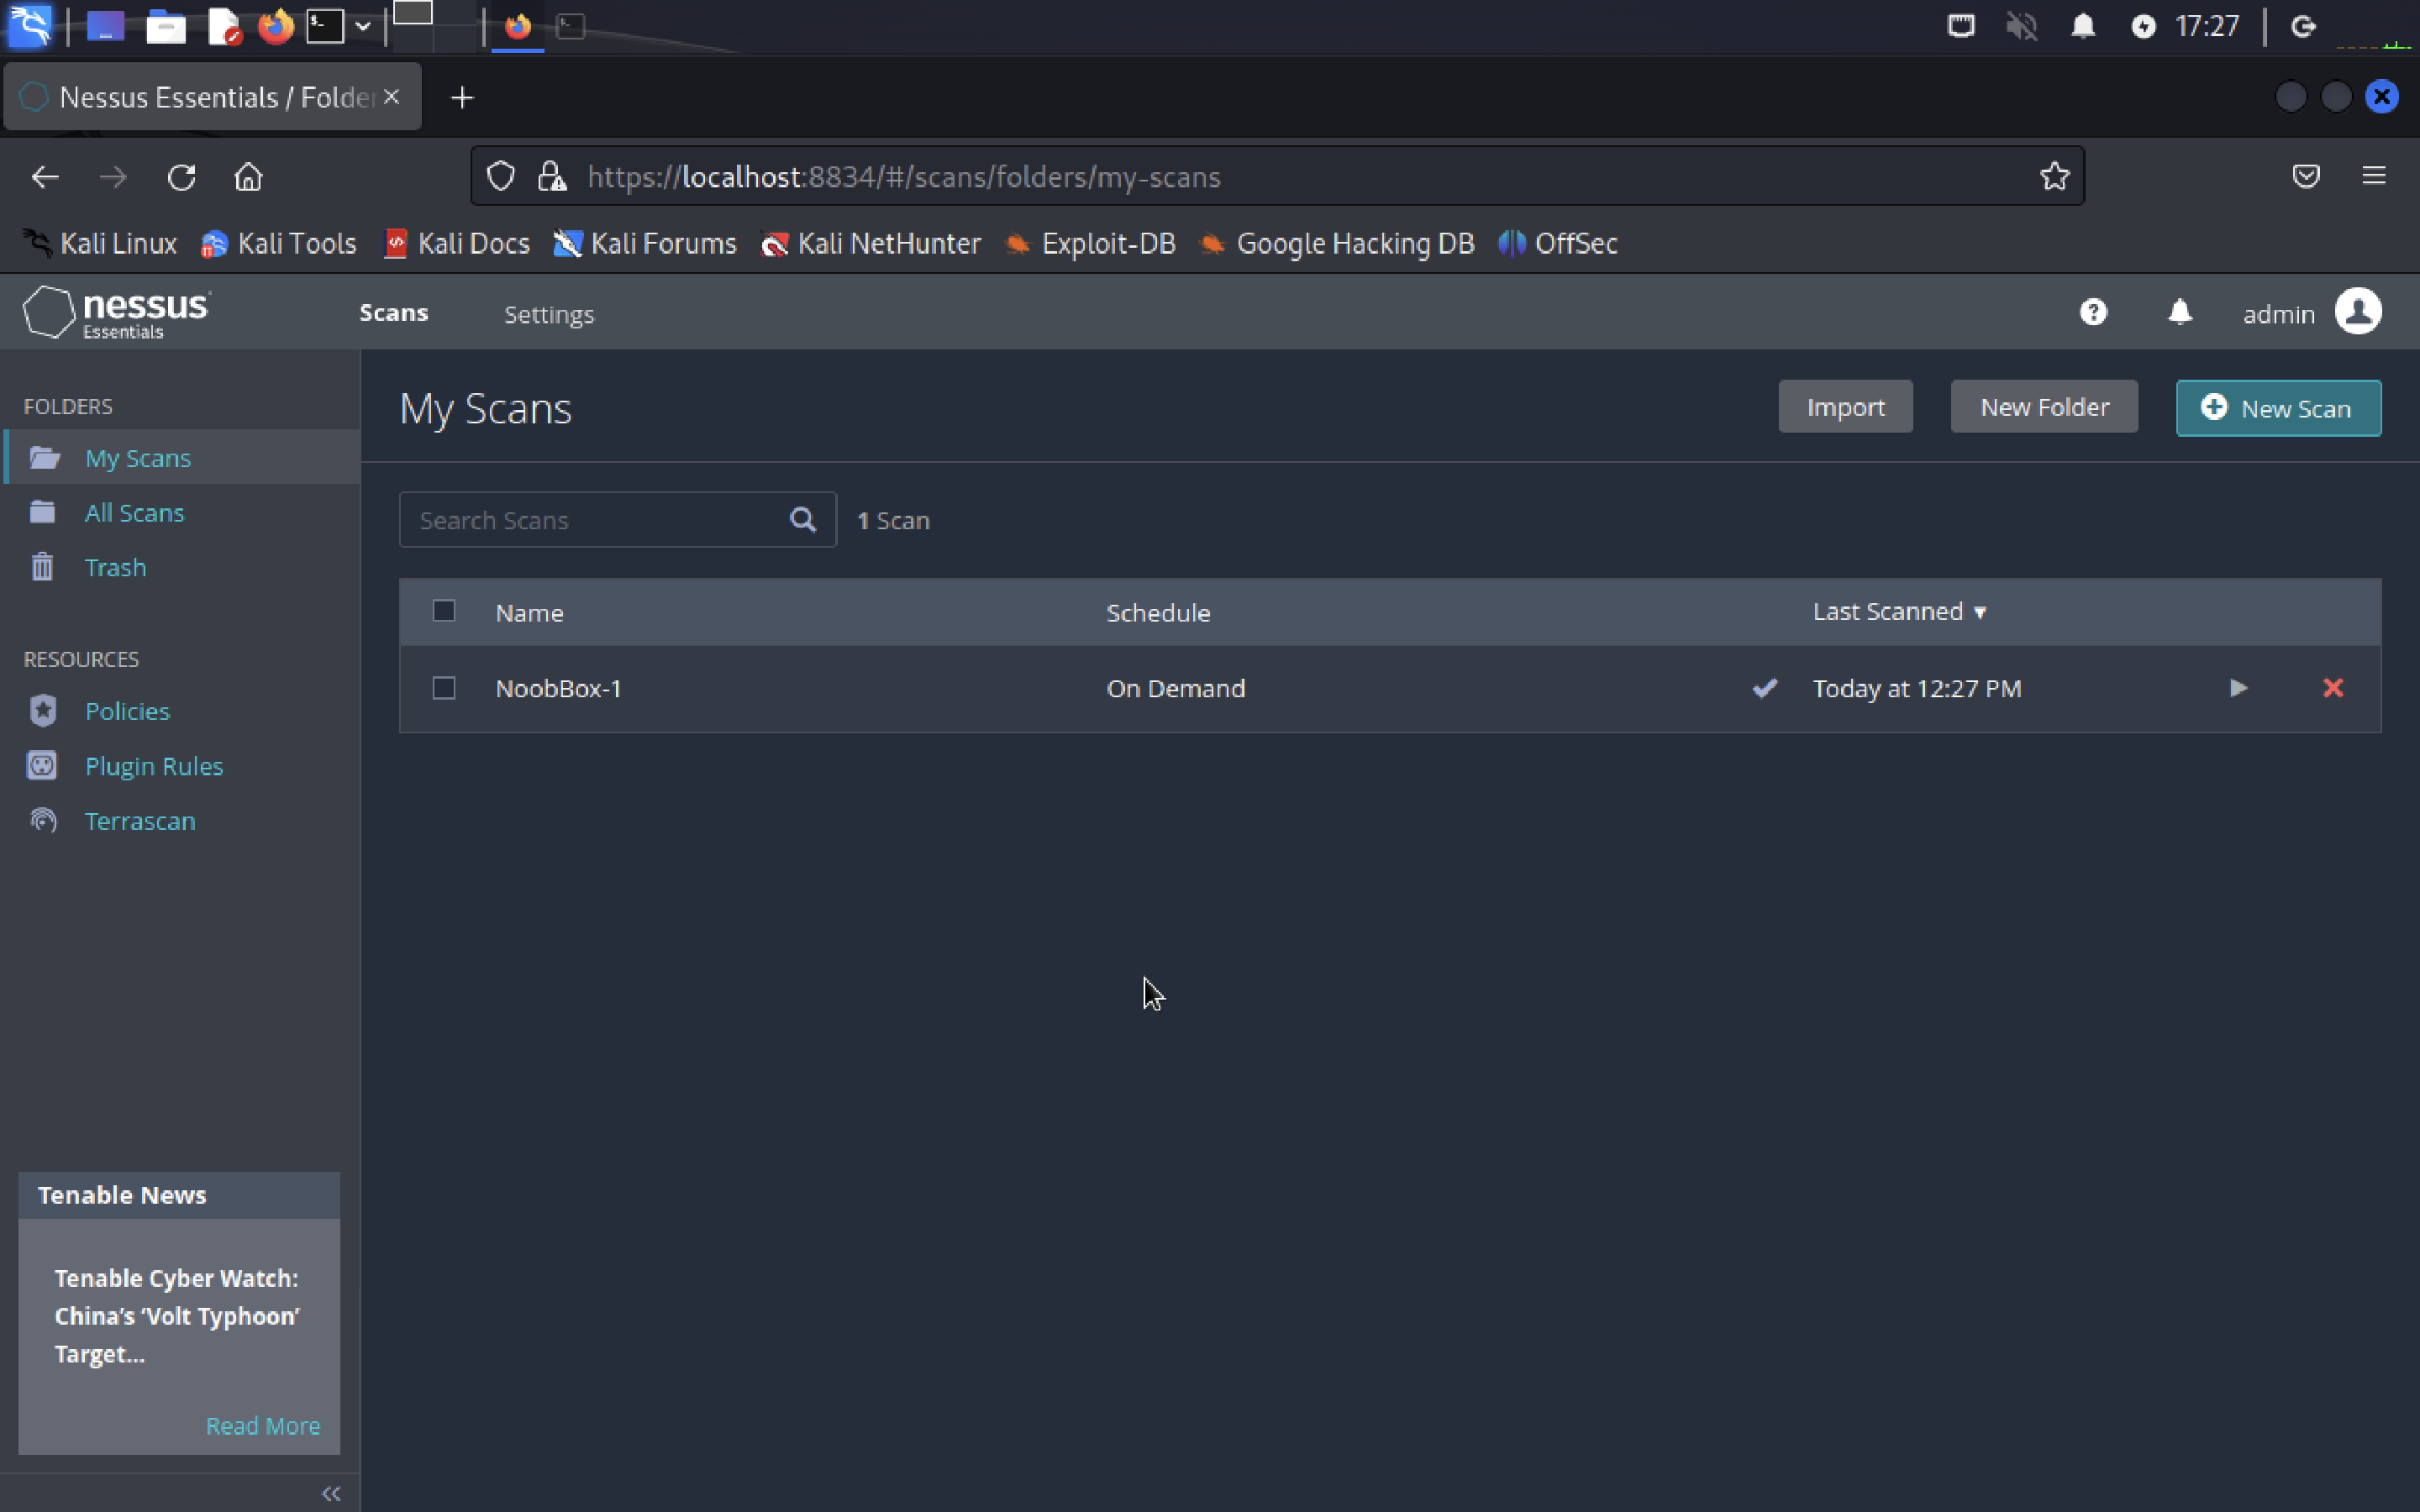
\includegraphics[width=\textwidth]{img/nessus-dashboard.png}
    \caption{La \textit{dashboard} di Nessus}
\end{figure}

La peculiarità di questo tool consiste nella presenza di diversi \textit{templates} di scansione, che si concentrano su determinati aspetta dell'asset da analizzare, come mostrato nella Figura 20.

\begin{figure}[h!]
    \centering
    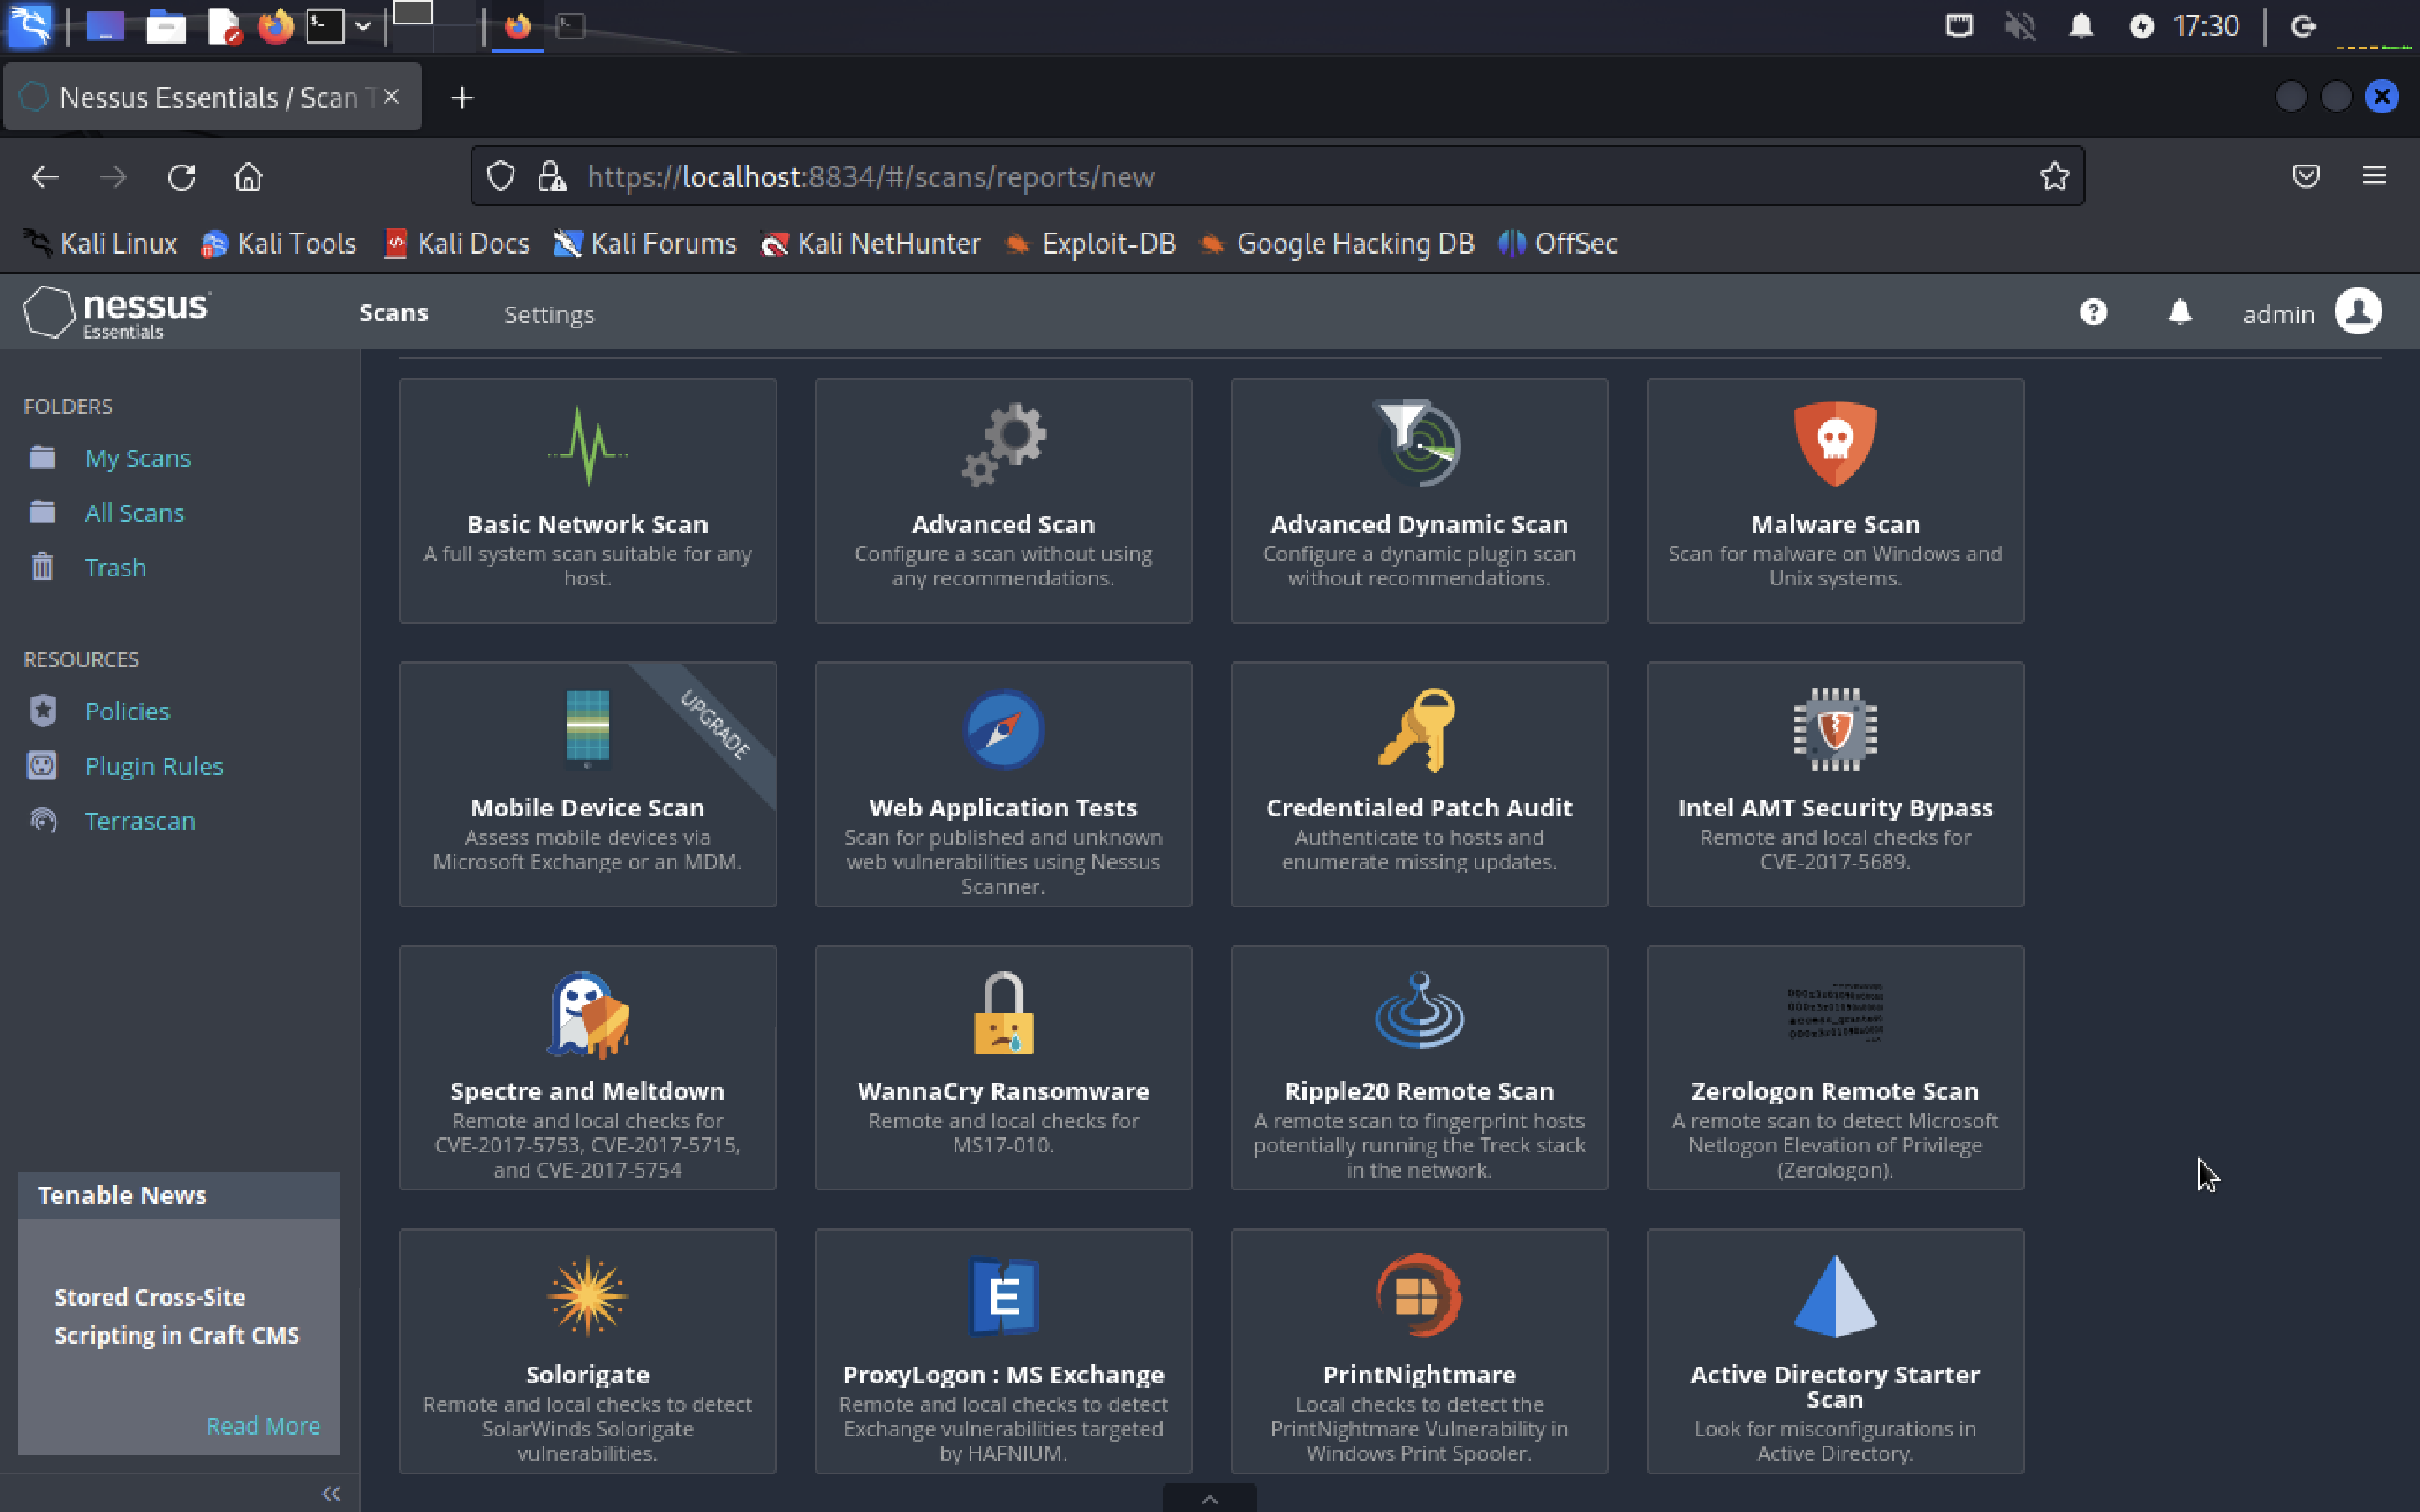
\includegraphics[width=\textwidth]{img/nessus-templates.png}
    \caption{I templates di Nessus}
\end{figure}

Per analizzare l'asset in esame, si è scelto di utilizzare il template \textbf{Web Application Tests}, che risulta quello più adatto per il contesto. Nel wizard che permette la definizione di una nuova scansione è stata selezionata la modalità \textbf{Complessa} che effettua le operazioni riportate nella Figura 21.

\begin{figure}[h!]
    \centering
    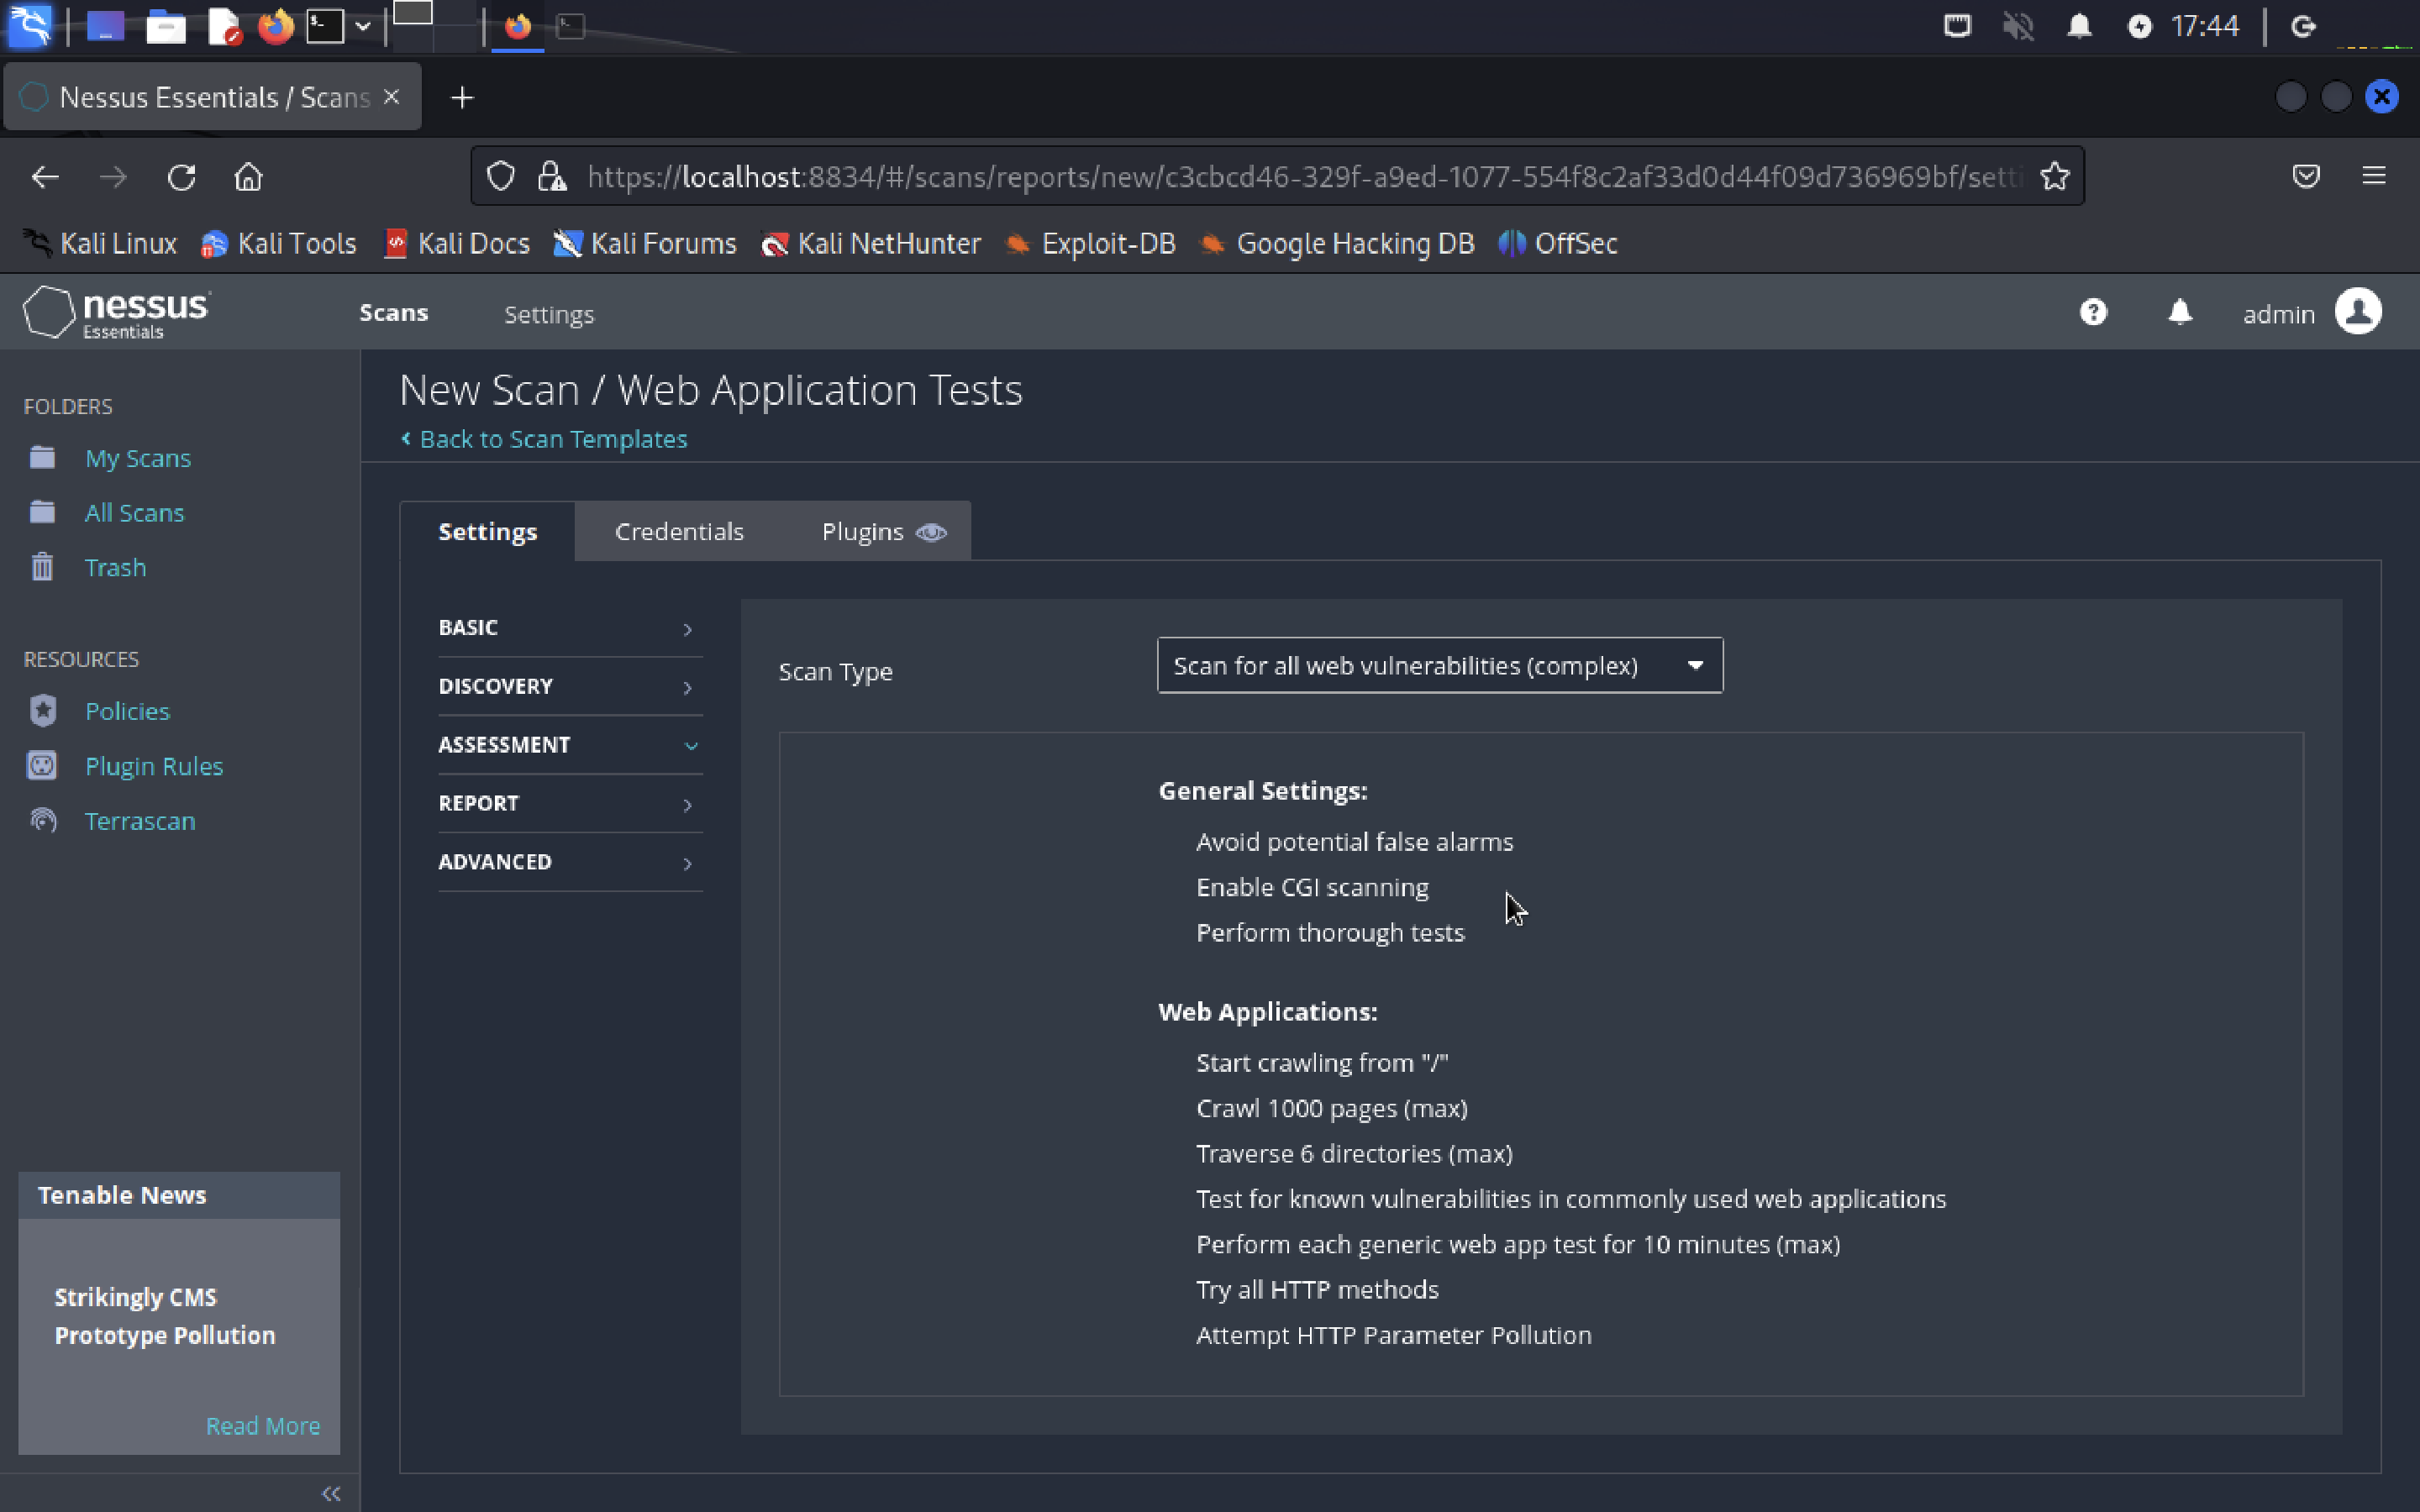
\includegraphics[width=\textwidth]{img/nessus-complex-scan.png}
    \caption{La scansione complessa di Nessus}
\end{figure}

\newpage
\subsubsection{Nessus: i risultati}
Al termine della scansione, Nessus fornisce un riepilogo delle vulnerabilità individuate e rappresentati mediante grafici, come mostrato nella Figura 22.

\begin{figure}[h!]
    \centering
    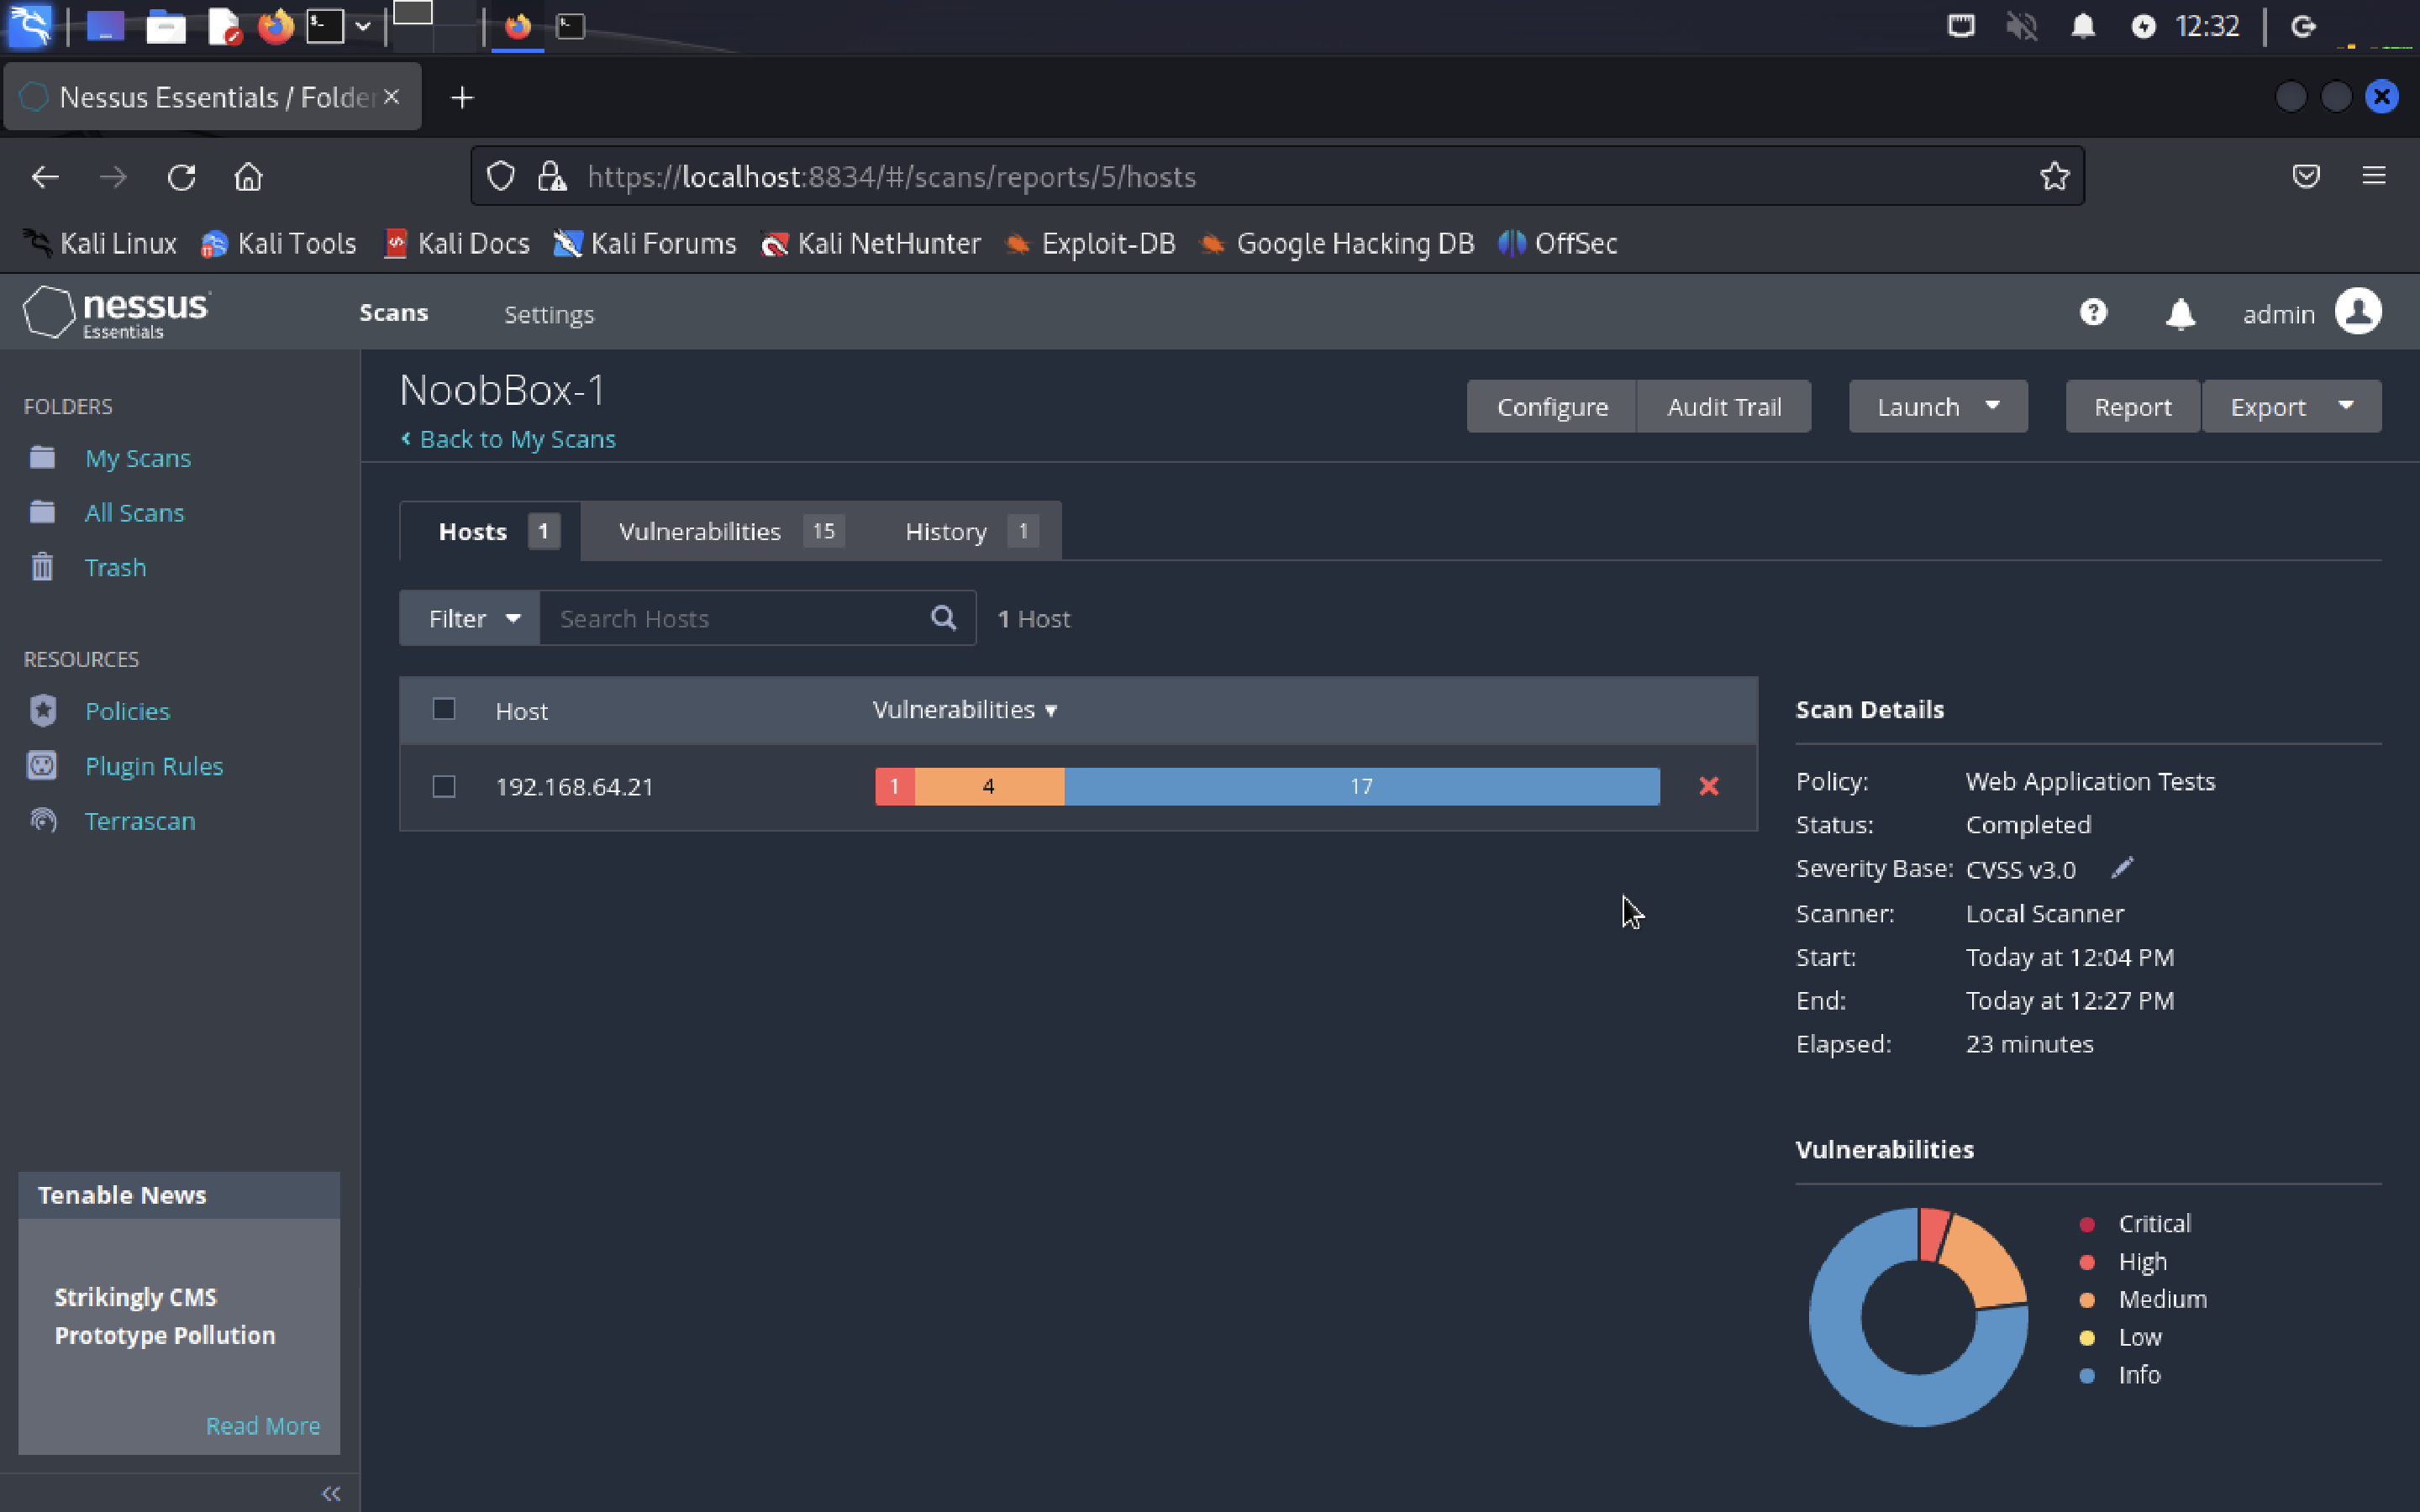
\includegraphics[width=\textwidth]{img/nessus-results.png}
    \caption{I risultati della scansione}
\end{figure}

Analizzando brevemente i risultati contenuti all'interno del file \texttt{Nessus-Scan.pdf}, allegato al Penetration Testing Report, si nota come Nessus abbia trovato (tralasciando qui i risultati di livello INFO) \textbf{cinque vulnerabilità}: una di livello \textbf{HIGH} e altre quattro di livello \textbf{MEDIUM}.

\subsubsection{Nota sulla vulnerabilità \textbf{HIGH}}
La vulnerabilità catalogata come di livello \textbf{HIGH} rappresenta in realtà un \textbf{falso positivo}. Facendo riferimento ai dettagli sul rilevamento, Nessus prova ad effettuare una \textbf{Server Side Includes (SSI) Injection} sulle pagine del \textbf{manuale del server} che spiegano come funziona questa tecnologia, tentando di includere una risorsa non esistente (e che quindi causerebbe un errore) e rilevando effettivamente un messaggio nel documento HTML di risposta che recita:

\begin{center}
    \texttt{[an error occurred while processing this directive]}
\end{center}

Tale messaggio è però \textit{hardcoded} all'interno del documento nella sezione che spiega come personalizzare proprio i messaggi di errore. Si può dunque ragionevolmente assumere che la Web App non sia vulnerabile a questo tipo di attacchi.

\subsubsection{Altre vulnerabilità}
Analizzando le altre vulnerabilità rilevate, si nota subito come sia stata confermata la possibilità di enumerare gli utenti di \textbf{WordPress}, già comunicata da \textbf{OpenVAS} e \texttt{wpscan}.
\newpage

\section{Target Exploitation}
Nelle sezioni precedenti di questo documento sono state raccolte informazioni utili da sfruttare nella fase di \textbf{Exploitation}. In particolare, nella fase di enumerazione è stato possibile rinvenire:

\begin{itemize}
    \item Lo \textbf{username} di un utente di Wordpress (\texttt{noobbox});
    \item Quella che sembra una \textbf{password} (rinvenuta nel file \textbf{/img.jpg}) nella root del server
\end{itemize}

Si suppone che queste credenziali siano valide per l'accesso di amministratore al framework Wordpress.

Poiché nella fase di \textbf{Vulnerability Mapping} non sono state rilevate altre vulnerabilità sfruttabili attivamente, la prima cosa che verrà provata nella fase di Exploitation sarà l'apertura di una shell sulla macchina con la suddetta coppia di credenziali \texttt{noobbox:5p4c3}. 
Una volta ottenuta una shell, verrà tentata una \textbf{Privilege Escalation} ed eventualmente l'installazione di una \textbf{backdoor} che permetta la permanenza dell'attaccante sulla macchina senza dover ripetere nuovamente l'exploit.

\subsection{Metasploit}
Il framework Metasploit è probabilmente il tool di Penetration Testing più usato che fornisce un modo semplice e veloce per eseguire exploit di varia natura su una moltitudine di tipologie di asset. Il framework è sviluppato e mantenuto da \textbf{Rapid7} ed è organizzato in \textbf{moduli} \cite{metasploit} che possono essere utilizzati per attaccare diverse tipologie di asset. Metasploit è presente di default su Kali Linux e il database dei moduli è reperibile al percorso \texttt{/usr/share/metasploit-framework/exploits}.

L'interazione col tool avviene mediante il comando

\begin{center}
    \texttt{msfconsole}
\end{center}

che permette l'apertura, appunto, di una \textbf{console} da cui è possibile richiamare i moduli mediante la direttiva

\begin{center}
    \texttt{use <path/del/modulo>}
\end{center}

I \textbf{parametri} dell'exploit sono invece impostabili mediante la direttiva

\begin{center}
    \texttt{set nome\_parametro valore\_parametro}
\end{center}

\subsection{Apertura di una shell}

Per questa analisi, verrà utilizzato il modulo \texttt{exploit/unix/webapp/wp\_admin\_shell\_upload}, che permette l'apertura di una \textbf{shell} di amministratore nel caso siano note le credenziali di accesso di \textbf{Wordpress}, come in questo caso.

Il payload che suddetto modulo usa è di tipo \textbf{reverse}, contenuto nel modulo \texttt{php/meterpreter/reverse\_tcp}, che permette apertura di una sessione \texttt{meterpreter} \footnote{\textbf{Meterpreter} è una shell che fornisce un gran numero di funzioni, tra cui l'upload di file sulla macchina target.\cite{meterpreter}}.

I parametri da impostare per questo exploit sono i seguenti:

\begin{itemize}
    \item \texttt{username}: l'username associato ad un utente Wordpress. In questo caso \texttt{noobbox};
    \item \texttt{password}: la password associata all'account di cui sopra. In questo caso \texttt{5p4c3};
    \item \texttt{rhost}: l'host su cui tentare l'exploit. In questo caso \texttt{192.168.64.21};
    \item \texttt{targeturi}: l'endpoint corrispondente alla root del sito web realizzato con wordpress. In questo caso \texttt{/wordpress/}.
\end{itemize}

Per lanciare l'exploit è sufficiente scrivere \texttt{exploit} nella console e premere Invio, come mostrato nella Figura 23.

\begin{figure}[h!]
    \centering
    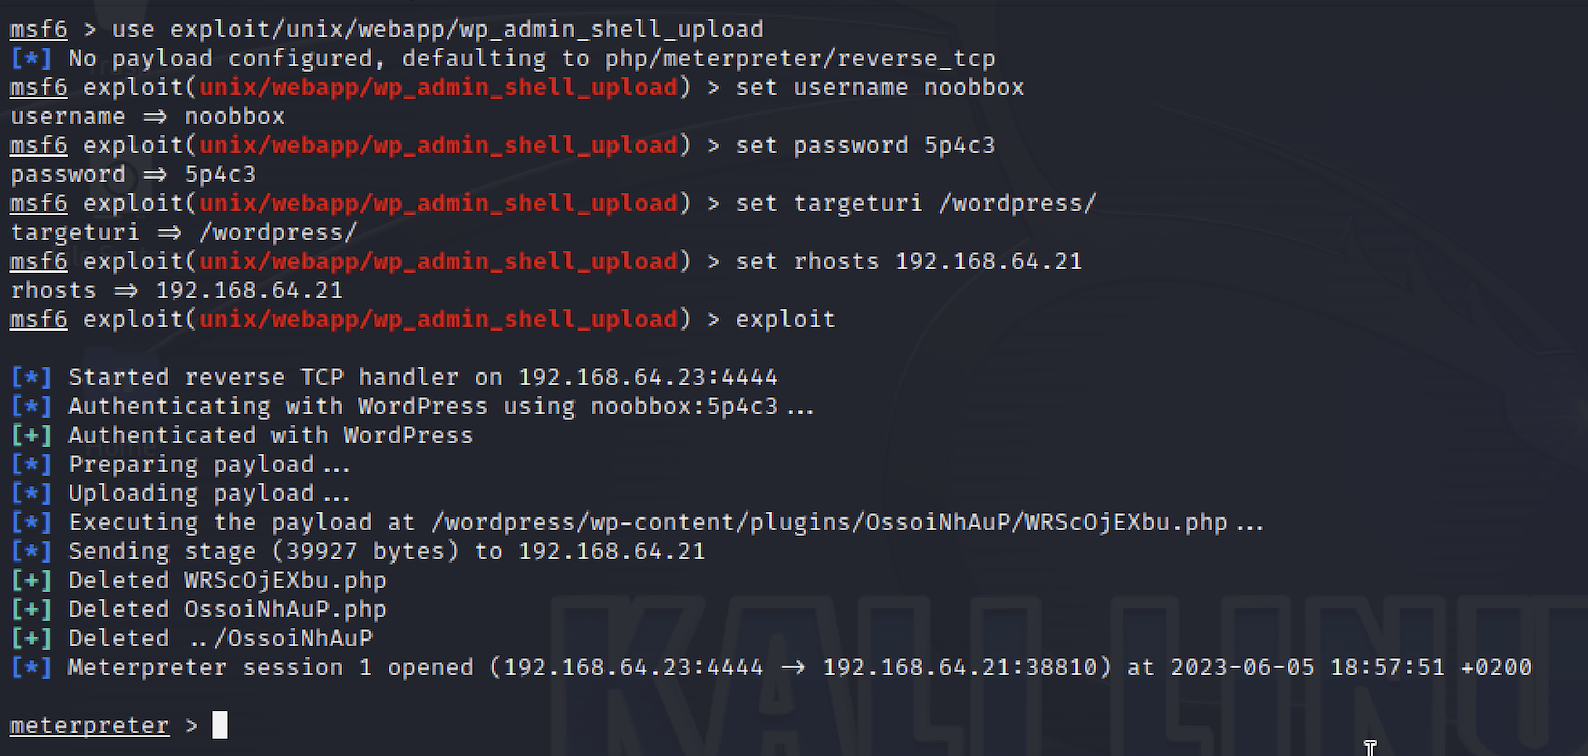
\includegraphics[width=\textwidth]{img/metaspolit_exploit.png}
    \caption{Esecuzione dell'exploit.}
\end{figure}

\newpage

Per accedere direttamente alla reverse shell aperta in un ambiente \textit{simil-xterm} è sufficiente eseguire il comando \texttt{shell -t} una volta giunti al prompt di \texttt{meterpreter}, come riportato nella Figura 24.

\begin{figure}[h!]
    \centering
    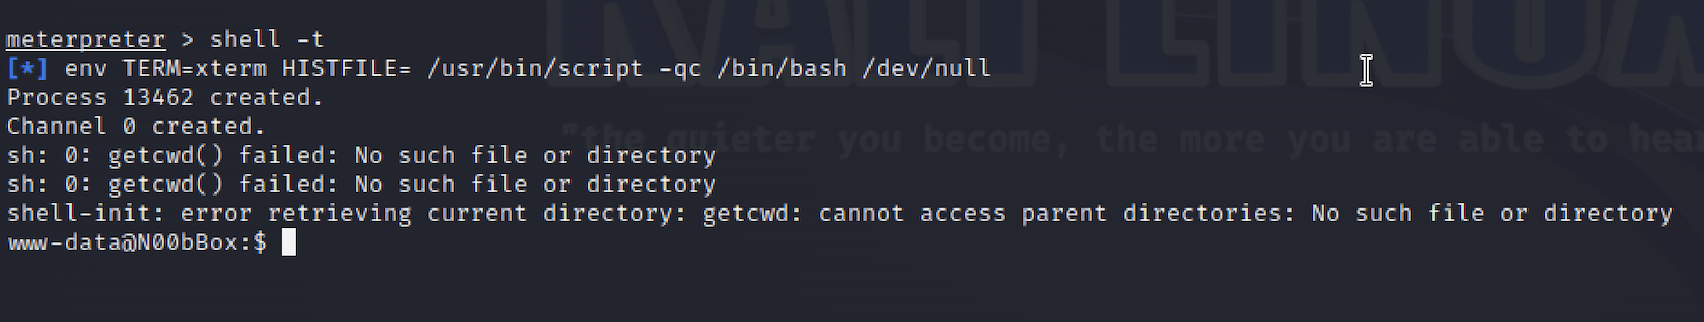
\includegraphics[width=\textwidth]{img/meterpreter-shell.png}
    \caption{Apertura di una shell.}
\end{figure}

L'intuizione relativa all'immagine rilevata in fase di enumerazione si è dimostrata quindi \textbf{corretta}: \texttt{5p4c3} rappresenta dunque una password valida per l'utente \texttt{noobbox}.

Allo stato attuale delle cose, si ha tuttavia a dispozione una shell per l'utente non privilegiato \texttt{www-data}. Tale account è utilizzato per convenzione per eseguire il server Apache \texttt{httpd}\cite{www-data}.

\newpage

\section{Privilege Escalation}
L'utente \texttt{www-data} \textbf{non è un utente privilegiato}. Lo scopo di questa fase è quindi tentare una \textbf{Privilege Escalation} ed ottenere l'accesso ad utenti "più privilegiati" e successivamente all'account \texttt{root}.

\newpage
\printbibliography[title={Riferimenti bibliografici e risorse consultate}]
\end{document}